\chapterauthor{Christopher Schieszler}
\chapter{Hardwareentwicklung, Schaltungstechnik und CAD-Konstruktion}
\label{chap:hardware}

Dieses Kapitel dokumentiert die vollständige elektronische und mechanische Neuentwicklung des \emph{Tumbler~v3.0}. Im ersten Teil werden der Schaltungsentwurf, die exakte Bauteildimensionierung sowie die Layout- und Regelprüfungen (ERC/DRC) der sechskanaligen Liniensensor-Platine und der überarbeiteten Hauptplatine behandelt. Der zweite Teil beschreibt die iterative 3D-CAD-Entwicklung des Unibody-Chassis bis zur druckfertigen Revision~v10.0, inklusive der fertigungsgerechten Auslegung (\gls{dfam}) für den \emph{Bambu Lab P1S}, der mechanischen Stoßfestigkeitsrechnung und der vollständigen Stückliste.

% ==============================================================================
\section{Neuentwicklung der Liniensensor-Platine (Layout R2)}
\label{sec:liniensensor_pcb}
% ==============================================================================
Die ursprünglich vorhandene Liniensensor-Schaltung aus der Vorjahresarbeit \cite{Kloeckl2026} wies mehrere gravierende Mängel auf: Die sechs optischen Reflexkoppler (\emph{CNY70}) waren über vier getrennte Steckverbinder (\texttt{J1}--\texttt{J4}) verdrahtet, es fehlten verbindliche Widerstandswerte für die Strombegrenzung und den Ausgangsteiler, und es existierte kein geprüftes Zweilagen-Layout mit durchgehender Massefläche. Im Rahmen dieser Diplomarbeit entstand daher das vollständig überarbeitete Paket \texttt{Liniensensor\_Redesign} (Schaltung~R1 / Layout~R2 in KiCad~9.0.9).

\subsection{Schaltungstopologie und Dimensionierung der IR-LED-Stromsenken}
Die sechs IR-Sendedioden der Reflexkoppler \texttt{U1}--\texttt{U6} (\emph{Vishay CNY70} \cite{Vishay_CNY70}) werden in zwei symmetrischen Dreier-Reihenschaltungen (\texttt{U1}--\texttt{U3} sowie \texttt{U4}--\texttt{U6}) direkt aus der geschalteten 2S-Akkuschiene \texttt{VBAT\_SW} (\qtyrange{6,4}{8,4}{\volt}) gespeist. Dadurch wird die \qty{3,3}{\volt}-Logikversorgung vollständig entlastet. Um den Diodenstrom trotz sinkender Akkuspannung weitgehend stabil bei rund \qty{20}{\milli\ampere} zu halten, steuert je ein NPN-Transistor \texttt{Q1}/\texttt{Q2} (\emph{Nexperia BC817-40,215}, SOT-23 \cite{Nexperia_BC817}) mit Emitterwiderstand $R_E = R_1 = R_9 = \qty{47}{\ohm}$ (\qty{1}{\percent}, 0805) als einfache Konstantstromsenke den Strangstrom.

Die Basisspannung wird über einen symmetrischen Spannungsteiler aus zwei \qty{1}{\kilo\ohm}-Widerständen (\texttt{R2}/\texttt{R3} bzw. \texttt{R7}/\texttt{R8}) aus den geregelten \qty{3,3}{\volt} gewonnen. Nach dem Satz von Thévenin ergeben sich die Leerlaufspannung $V_{\mathrm{th}}$ und der Innenwiderstand $R_{\mathrm{th}}$ der Basisquelle zu \cite{TietzeSchenk}:
\begin{equation}
  V_{\mathrm{th}} = \frac{\qty{3,3}{\volt}}{2} = \qty{1,65}{\volt}, \qquad
  R_{\mathrm{th}} = \qty{1}{\kilo\ohm} \parallel \qty{1}{\kilo\ohm} = \qty{500}{\ohm}
  \label{eq:ls_thevenin}
\end{equation}
Unter Berücksichtigung der Stromverstärkung $\beta$ und der Basis-Emitter-Flussspannung $V_{BE}$ folgt für den Kollektorstrom $I_C$ (identisch mit dem IR-LED-Strom $I_F$ jeder der drei in Serie liegenden Dioden):
\begin{equation}
  I_C = \frac{V_{\mathrm{th}} - V_{BE}}{R_E \cdot \left(1 + \frac{1}{\beta}\right) + \frac{R_{\mathrm{th}}}{\beta}}
  \label{eq:ls_stromsenke}
\end{equation}
Für typische Werte eines \emph{BC817-40} ($\beta = 200$, $V_{BE} = \qty{0,65}{\volt}$) ergibt sich:
\begin{equation}
  I_C = \frac{\qty{1,65}{\volt} - \qty{0,65}{\volt}}{\qty{47}{\ohm} \cdot 1{,}005 + \frac{\qty{500}{\ohm}}{200}} = \frac{\qty{1,00}{\volt}}{\qty{49,735}{\ohm}} = \qty{20,11}{\milli\ampere}
  \label{eq:ls_ic_nom}
\end{equation}
Bei $V_{BE} = \qty{0,70}{\volt}$ sinkt der Strom geringfügig auf \qty{19,10}{\milli\ampere}. Beide Stränge zusammen entnehmen somit rund \qty{40}{\milli\ampere} aus \texttt{VBAT\_SW} -- weit unter dem absoluten Grenzstrom der CNY70-LED (\qty{50}{\milli\ampere}).

\subsubsection{Verlustleistungs- und Grenzfallanalyse (6,4 V bis 8,4 V)}
Bei voll geladenem 2S-Akku ($U_{\mathrm{Bat}} = \qty{8,4}{\volt}$) und einer typischen IR-LED-Flussspannung von $V_F \approx \qty{1,25}{\volt}$ pro Diode ($3 \times \qty{1,25}{\volt} = \qty{3,75}{\volt}$) verbleibt über Emitterwiderstand und Transistor eine Spannung von $\qty{8,4}{\volt} - \qty{3,75}{\volt} = \qty{4,65}{\volt}$. Die entstehenden Verlustleistungen liegen weit innerhalb der zulässigen Bauteilgrenzen \cite{Vishay_CRCW,Nexperia_BC817}:
\begin{align}
  P_{R1,R9} &= I_E^2 \cdot R_E \approx (\qty{20,2}{\milli\ampere})^2 \cdot \qty{47}{\ohm} = \qty{19,2}{\milli\watt} \quad (\text{Nennwert: } \qty{125}{\milli\watt}) \label{eq:ls_p_re} \\
  P_{Q1,Q2} &= U_{CE} \cdot I_C \approx (\qty{4,65}{\volt} - \qty{0,95}{\volt}) \cdot \qty{20,11}{\milli\ampere} = \qty{74,4}{\milli\watt} \quad (\text{Nennwert: } \qty{250}{\milli\watt}\text{ bei }\qty{25}{\celsius}) \label{eq:ls_p_q}
\end{align}
Selbst in einer konservativen Worst-Case-Parameterstudie (\qty{3,3}{\volt} $\pm 5\,\%$, Widerstände $\pm 1\,\%$, $\beta \in [100, 600]$, $V_{BE} \in [\qty{0,5}{\volt}, \qty{0,9}{\volt}]$, $V_F \in [\qty{0,9}{\volt}, \qty{1,6}{\volt}]$) bleibt der Strangstrom im Bereich \qtyrange{12,3}{26,3}{\milli\ampere} und die maximale Transistorverlustleistung bei \qty{117,8}{\milli\watt} (bei \qty{60}{\celsius} Umgebungstemperatur stehen mit $R_{\mathrm{thJA}} = \qty{500}{\kelvin\per\watt}$ noch \qty{180}{\milli\watt} zur Verfügung). Bei entladenem Akku (\qty{6,4}{\volt}) und konservativen $3 \times \qty{1,6}{\volt} = \qty{4,8}{\volt}$ verbleiben noch rund \qty{0,6}{\volt} Kollektor-Emitter-Spannung, sodass die Stromsenken über das gesamte 2S-Spannungsfenster arbeiten.

\subsection{Ausgangs-Spannungsteiler, ADC-Anpassung und RC-Tiefpassfilter}
Ein kritisches Detail bei der direkten Anbindung an den \emph{ESP32-S3} ist der kalibrierte Messbereich des integrierten 12-Bit-ADCs (\texttt{ADC1}): Selbst bei maximaler interner Dämpfung (\qty{11}{\decibel} bzw. \qty{12}{\decibel}) spezifiziert Espressif den linear kalibrierten Bereich nur bis ca. \qty{2,9}{\volt} \cite{EspressifESP32S3}. Würde man den Phototransistor-Kollektor lediglich mit einem Pull-up nach \qty{3,3}{\volt} verbinden, läge der Dunkelwert über einer schwarzen Linie bei \qty{3,3}{\volt} und damit in der ADC-Sättigung.

Deshalb wurde jeder der sechs Kanäle (\texttt{LS1}--\texttt{LS6}) mit einem Ausgangs-Spannungsteiler aus Pull-up $R_{\mathrm{up}} = \qty{10}{\kilo\ohm}$ (\texttt{R4}--\texttt{R6}, \texttt{R10}--\texttt{R12}) nach \qty{3,3}{\volt}, Pull-down $R_{\mathrm{down}} = \qty{47}{\kilo\ohm}$ (\texttt{R13}--\texttt{R18}) nach \texttt{GND} sowie einem Filterkondensator $C_F = \qty{10}{\nano\farad}$ (\texttt{C5}--\texttt{C10}, 0805 X7R \qty{50}{\volt}) gegen \texttt{GND} beschaltet. Alle Emitter liegen direkt auf \texttt{GND}. Daraus berechnen sich der nominale Dunkelwert ($I_{\mathrm{Photo}} = 0$), der effektive Quellenwiderstand $R_{\mathrm{eq}}$ und die Tiefpass-Grenzfrequenz $f_g$:
\begin{align}
  U_{\mathrm{Dunkel,nom}} &= \qty{3,3}{\volt} \cdot \frac{\qty{47}{\kilo\ohm}}{\qty{10}{\kilo\ohm} + \qty{47}{\kilo\ohm}} = \qty{2,721}{\volt} \label{eq:ls_udunkel} \\
  R_{\mathrm{eq}} &= \qty{10}{\kilo\ohm} \parallel \qty{47}{\kilo\ohm} = \frac{10 \cdot 47}{10 + 47}\,\mathrm{k\Omega} = \qty{8,246}{\kilo\ohm} \label{eq:ls_req} \\
  \tau &= R_{\mathrm{eq}} \cdot C_F = \qty{8,246}{\kilo\ohm} \cdot \qty{10}{\nano\farad} = \qty{82,5}{\micro\second} \label{eq:ls_tau} \\
  f_g &= \frac{1}{2\pi \cdot \tau} = \frac{1}{2\pi \cdot \qty{82,5}{\micro\second}} \approx \qty{1,93}{\kilo\hertz} \label{eq:ls_fg}
\end{align}
Vor Erreichen der Transistorsättigung folgt die Kanalspannung näherungsweise $U_{\mathrm{LS}} \approx \qty{2,721}{\volt} - I_{\mathrm{Photo}} \cdot \qty{8,246}{\kilo\ohm}$. Selbst im ungünstigsten Toleranzfall ($+5\,\%$ Versorgungsspannung, $\pm 1\,\%$ Widerstände) erreicht der Dunkelwert maximal \qty{2,867}{\volt} und bleibt damit sicher unterhalb der \qty{2,9}{\volt}-ADC-Grenze. Gleichzeitig dämpft der \qty{1,93}{\kilo\hertz}-Tiefpass eingekoppelte Motor-PWM-Störungen bei \qty{20}{\kilo\hertz} bereits um über \qty{20}{\decibel}, während die Sprungantwort ($\approx 5\tau = \qty{0,41}{\milli\second}$) bei einer Fahrgeschwindigkeit von \qty{1}{\meter\per\second} einer Wegauflösung von nur \qty{0,41}{\milli\meter} entspricht. Abbildung~\ref{fig:cny70_transfer} stellt beide Kennlinien grafisch dar.

\begin{figure}[htbp]
  \centering
  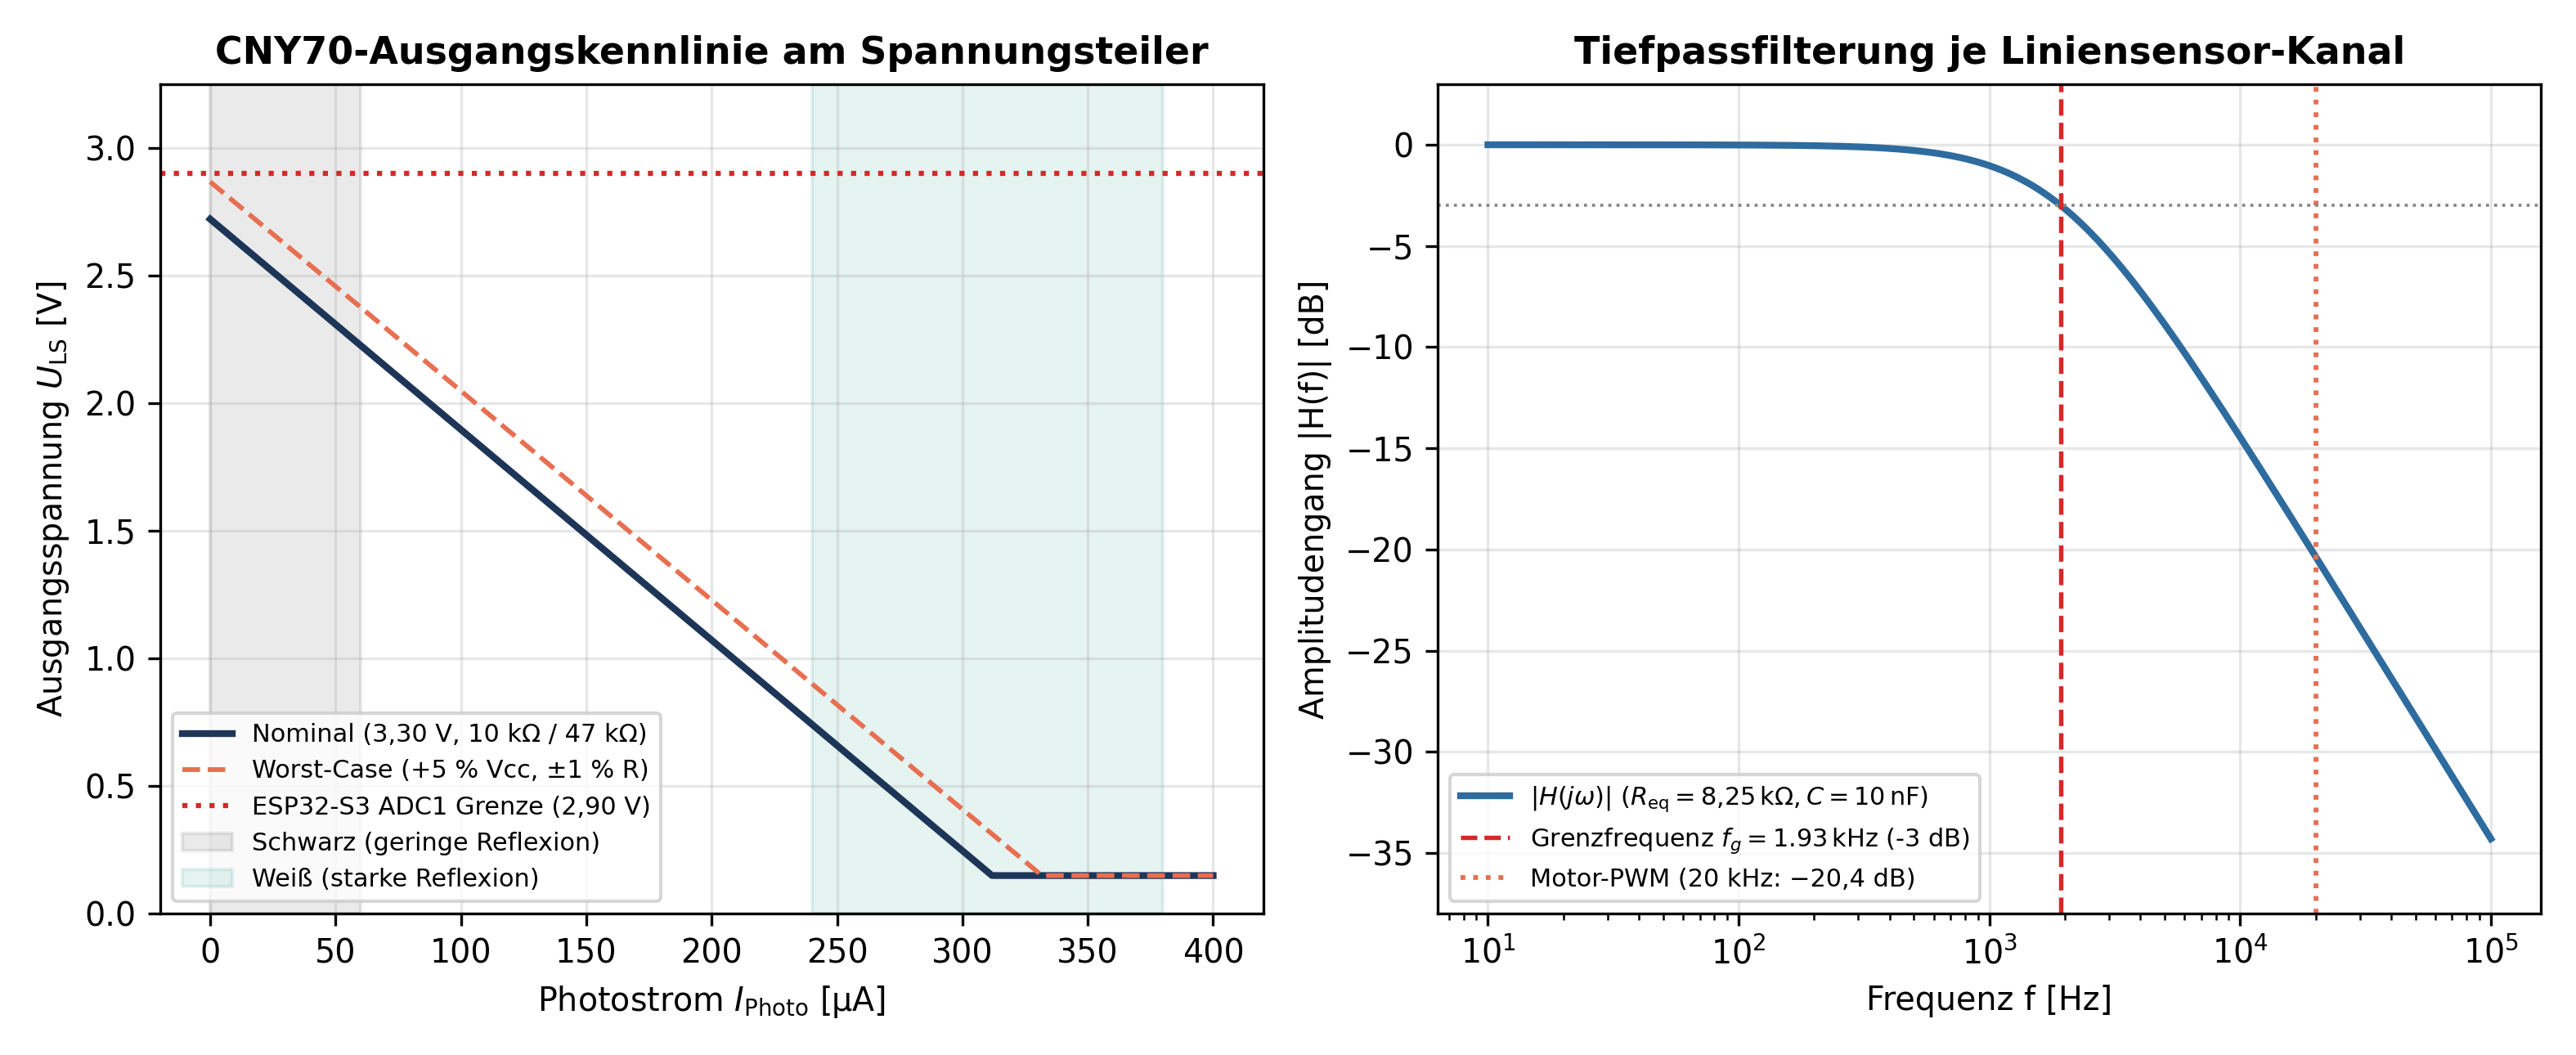
\includegraphics[width=0.98\textwidth]{figures/fig_cny70_transfer_rc.png}
  \caption{Berechnete Ausgangskennlinie $U_{\mathrm{LS}}(I_{\mathrm{Photo}})$ (links) und Tiefpass-Amplitudengang $|H(f)|$ (rechts) der Liniensensor-Platine R2.}
  \label{fig:cny70_transfer}
\end{figure}

\subsection{PCB-Layout, Höhenkette und KiCad-Regelprüfung (ERC/DRC)}
Die Leiterplatte wurde zweilagig in FR4 (\qtyproduct{76 x 32 x 1,6}{\milli\meter}, \qty{35}{\micro\meter} Kupferauflage, vier \qty{3,2}{\milli\meter}-NPTH-Bohrungen im Raster \qtyproduct{68 x 24}{\milli\meter}) geroutet. Sämtliche SMD-Komponenten (0805/1206-Widerstände und -Kondensatoren, SOT-23-Transistoren, seitlicher 10-poliger JST-GH-Steckverbinder \texttt{J2} \cite{JST_GH}) sitzen auf der Oberseite (\texttt{F.Cu}), während die sechs \emph{CNY70}-Sensoren im \qty{10}{\milli\meter}-Raster auf der Unterseite (\texttt{B.Cu}) mit Blickrichtung Fahrbahn bestückt werden. Die Unterseite trägt eine großflächige, geschlossene Massefläche (\texttt{GND}) mit kupferfreien Sperrzonen um die vier M3-Schraubköpfe.

\begin{figure}[htbp]
  \centering
  \begin{subfigure}[b]{0.48\textwidth}
    \centering
    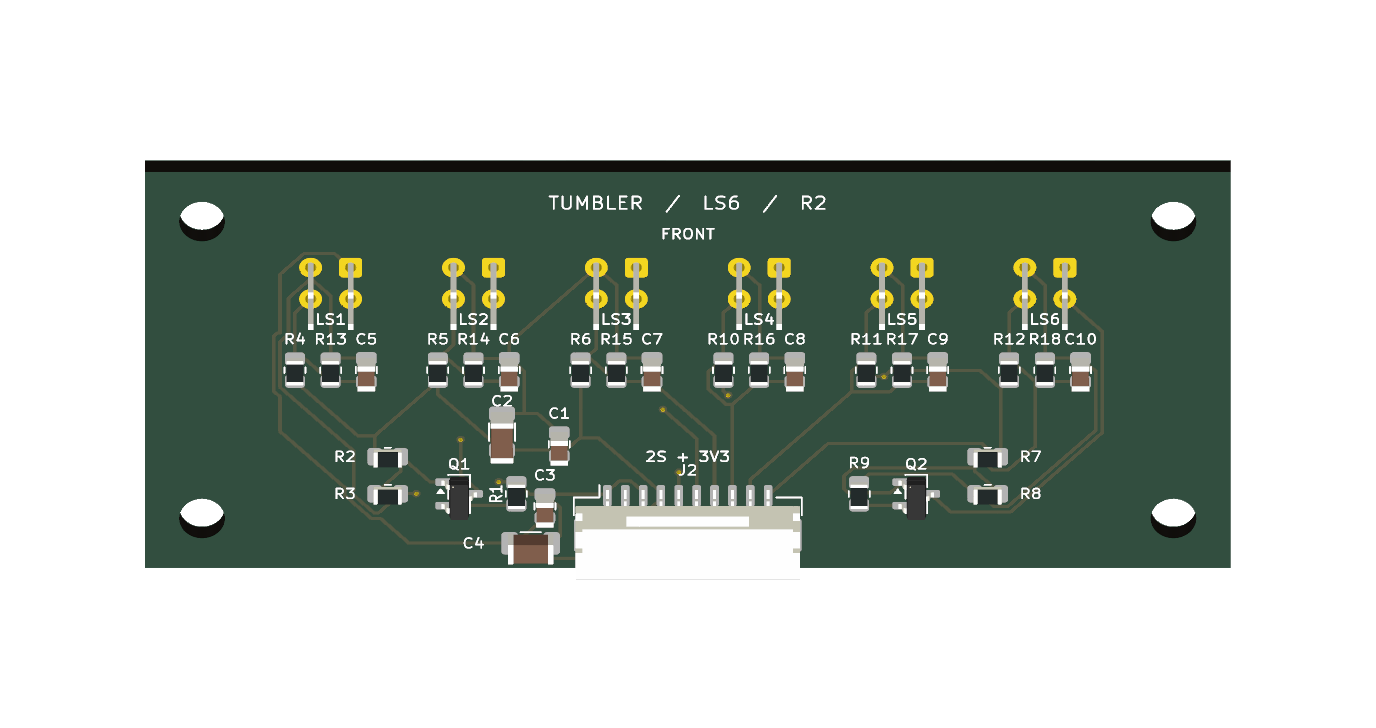
\includegraphics[width=\textwidth]{figures/pcb_ls_oben.png}
    \caption{Oberseite (\texttt{F.Cu}): SMD-Filter, Stromsenken \& JST-GH.}
    \label{fig:pcb_ls_oben}
  \end{subfigure}
  \hfill
  \begin{subfigure}[b]{0.48\textwidth}
    \centering
    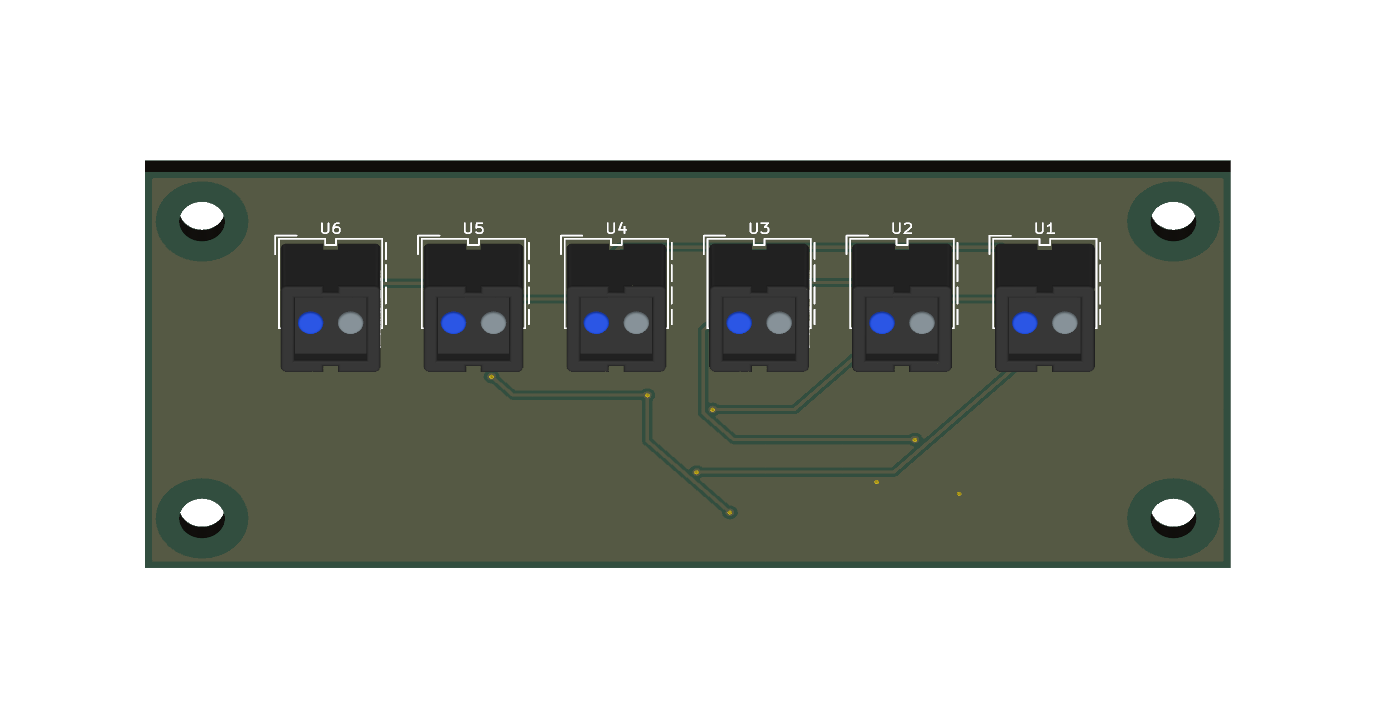
\includegraphics[width=\textwidth]{figures/pcb_ls_unten.png}
    \caption{Unterseite (\texttt{B.Cu}): 6$\times$ CNY70 im \qty{10}{\milli\meter}-Raster.}
    \label{fig:pcb_ls_unten}
  \end{subfigure}
  \caption{3D-CAD-Ansichten der neu gerouteten Liniensensor-Platine R2 (\qtyproduct{76 x 32}{\milli\meter}) aus KiCad.}
  \label{fig:pcb_ls_views}
\end{figure}

Ein praxisnahes Detail ergab sich beim Electrical Rules Check (\gls{erc}): Das offizielle KiCad-Standardsymbol des \emph{CNY70} deklariert den Phototransistor-Emitter (Pin~4) als \texttt{open\_emitter}, was bei direkter Masseanbindung sechs künstliche Pin-Typ-Konflikte mit dem \texttt{PWR\_FLAG} erzeugt. Statt die ERC-Regel blind abzuschalten, wurde eine projektlokale Symbolkopie (\texttt{Tumbler\_Sensor.kicad\_sym}) angelegt, die Pin~4 elektrisch korrekt als passiven Transistoranschluss führt. Die abschließende Prüfung in KiCad~9.0.9 (37 elektrische Bauteile, 19 Netze, \qty{0,25}{\milli\meter} Leiterbahnbreite, \qty{0,20}{\milli\meter} Mindestabstand, \qty{0,60}/\qty{0,30}{\milli\meter} Vias) schloss mit **0 ERC-Fehlern, 0 ERC-Warnungen und 0 DRC-Verletzungen** ab.

Für die mechanische Integration gilt eine definierte Höhenkette: Bei einem optischen Arbeitsabstand von \qty{2,0}{\milli\meter} über der Fahrbahn, \qty{6,0}{\milli\meter} Bauhöhe des CNY70-Gehäuses und \qty{0,5}{\milli\meter} Löt-Sitzabstand liegt die PCB-Unterseite auf \qty{8,5}{\milli\meter} und die Oberseite auf \qty{10,1}{\milli\meter} über Boden. Abbildung~\ref{fig:pcb_ls_halter} zeigt den für erste Vorversuche erstellten Prüfhalter; im finalen Unibody-Chassis~v10.0 wird die Platine direkt von unten gegen den \qty{8,0}{\milli\meter} starken Frontflansch verschraubt.

\begin{figure}[htbp]
  \centering
  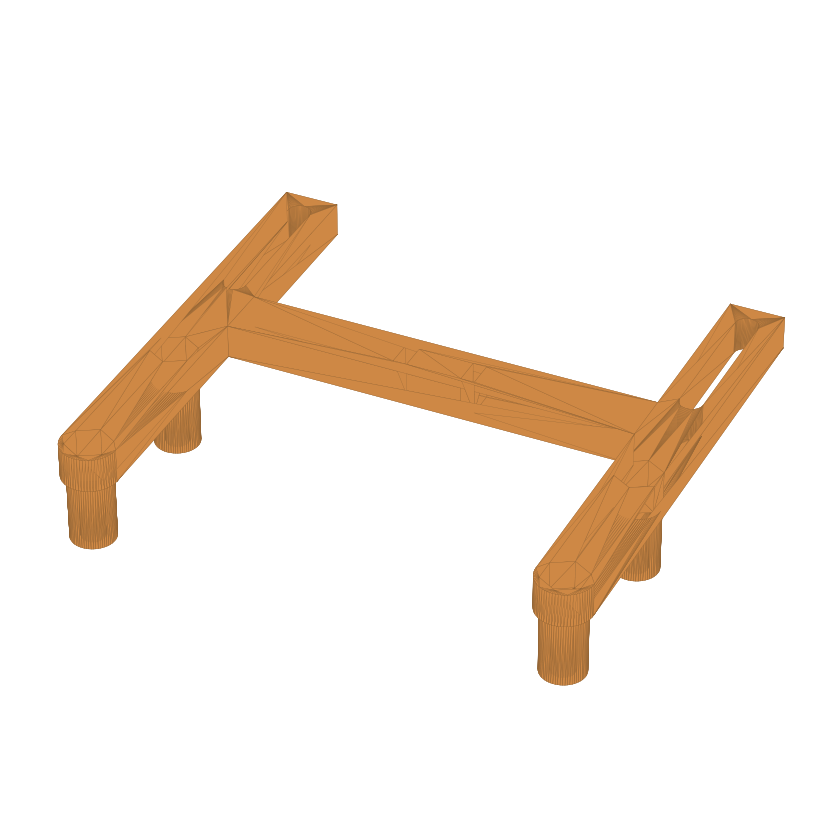
\includegraphics[width=0.58\textwidth]{figures/pcb_ls_halter.png}
  \caption{Mechanische CAD-Ansicht des Prototyp-Sensorhalters für Vorversuche am Liniensensor.}
  \label{fig:pcb_ls_halter}
\end{figure}

% ==============================================================================
\section{Hauptplatine (Tumbler2\_Redesign -- Stufe 1 Signalteil)}
\label{sec:hauptplatine}
% ==============================================================================
Parallel zur Liniensensor-Platine wurde der Schaltplan der Hauptplatine (\texttt{Tumbler2\_Redesign}, \qtyproduct{76,962 x 80,518 x 1,60}{\milli\meter}, M3-Bohrraster \qtyproduct{65,0 x 64,0}{\milli\meter}) in KiCad~10 strukturell bereinigt und auf die neue Sensorik abgestimmt. Der Entwurf wurde bewusst in zwei klar abgegrenzte Ausbaustufen unterteilt: \emph{Stufe~1} (Signalteil, Busgruppen, MCU-Pinzuordnung und geprüfte Netzliste) sowie \emph{Stufe~2} (Leistungspfad, 2S-Ladeschaltung, Verpolschutz und finale Bauteilfestlegung).

\subsection{Wesentliche Änderungen im Signalteil (Stufe 1)}
Gegenüber dem ursprünglichen Arbeitsstand wurden folgende Verbesserungen umgesetzt und durch 51 automatisierte Netzlistenprüfungen (alle 51 \texttt{PASS}) abgesichert:
\begin{itemize}
  \item \textbf{Explizite Busgruppen:} Alle Hierarchie-Übergänge wurden sauber typisiert (\texttt{USB:\{DN DP\}}, \texttt{I2C:\{SDA SCL\}}, \texttt{Motor A:\{AIN1 AIN2 ENCA\_A ENCB\_A\}} und \texttt{Motor B:\{BIN1 BIN2 ENCA\_B ENCB\_B\}}).
  \item \textbf{1:1-Anbindung des Liniensensors (\texttt{J2}):} Ein vertikaler 10-poliger JST-GH-Steckverbinder (\texttt{BM10B-GHS-TBT}) verbindet die sechs Kanäle \texttt{LS1}--\texttt{LS6} über je einen \qty{100}{\ohm}-Serien-Schutzwiderstand (\texttt{R3}, \texttt{R4}, \texttt{R29}--\texttt{R32}, 0603, \qty{0,1}{\watt}) direkt mit sechs Kanälen des \texttt{ADC1} am ESP32-S3 (Tabelle~\ref{tab:j2_pinout}). Die \qty{100}{\ohm}-Widerstände schützen die GPIO-Eingänge vor ESD und kapazitiven Umladespitzen, ohne die \qty{8,25}{\kilo\ohm}-Quellenimpedanz der Sensorplatine nennenswert zu verfälschen.
  \item \textbf{Konfliktfreie Pin-Umschichtung:} Da \texttt{GPIO9} und \texttt{GPIO10} nun für \texttt{LS5} und \texttt{LS6} auf \texttt{ADC1} reserviert sind, wurden der Benutzertaster auf \texttt{GPIO15} und das optionale Echo-Signal auf \texttt{GPIO16} verlegt.
  \item \textbf{USB-C- und LED-Korrektur:} Die USB-Datenleitungen erhielten \qty{22}{\ohm}-Serienwiderstände (\texttt{R33}, \texttt{R34}, 0603) unmittelbar am ESP32-S3 gemäß Espressif-Design-Guideline \cite{EspressifHWGuide}. Bei \texttt{R28} wurde ein fehlerhafter \qty{5}{\volt}-Pull-up gegen einen \qty{10}{\kilo\ohm}-Pulldown nach \texttt{GND} ersetzt.
\end{itemize}

\begin{table}[htbp]
\centering
\caption{1:1-Steckerbelegung von \texttt{J2} (10-pol. JST GH) zwischen Liniensensor und Hauptplatine.}
\label{tab:j2_pinout}
\begin{tabular}{@{}c l c c l@{}}
\toprule
\textbf{Pin J2} & \textbf{Netzname} & \textbf{ESP32-S3 GPIO} & \textbf{ADC-Kanal} & \textbf{Funktion / Hinweis} \\
\midrule
1 & \texttt{GND} & -- & -- & Hauptmasse (Rückleitung) \\
2 & \texttt{VBAT\_SW} & -- & -- & Geschaltete 2S-Akkuspannung (\qtyrange{6,4}{8,4}{\volt}) \\
3 & \texttt{GND} & -- & -- & Zweite Masseleitung (Sensor-Referenz) \\
4 & \texttt{+3.3V} & -- & -- & Geregelte \qty{3,3}{\volt}-Versorgung \\
5 & \texttt{LS1} & \texttt{GPIO4} & \texttt{ADC1\_CH3} & CNY70 \texttt{U1} (links außen), über \qty{100}{\ohm} (\texttt{R3}) \\
6 & \texttt{LS2} & \texttt{GPIO5} & \texttt{ADC1\_CH4} & CNY70 \texttt{U2}, über \qty{100}{\ohm} (\texttt{R4}) \\
7 & \texttt{LS3} & \texttt{GPIO6} & \texttt{ADC1\_CH5} & CNY70 \texttt{U3} (links Mitte), über \qty{100}{\ohm} (\texttt{R29}) \\
8 & \texttt{LS4} & \texttt{GPIO7} & \texttt{ADC1\_CH6} & CNY70 \texttt{U4} (rechts Mitte), über \qty{100}{\ohm} (\texttt{R30}) \\
9 & \texttt{LS5} & \texttt{GPIO9} & \texttt{ADC1\_CH8} & CNY70 \texttt{U5}, über \qty{100}{\ohm} (\texttt{R31}) \\
10 & \texttt{LS6} & \texttt{GPIO10} & \texttt{ADC1\_CH9} & CNY70 \texttt{U6} (rechts außen), über \qty{100}{\ohm} (\texttt{R32}) \\
\bottomrule
\end{tabular}
\end{table}

Abbildung~\ref{fig:pcb_main_sch} zeigt die überarbeiteten Schaltplanseiten des Mikrocontroller- und LED-Teils aus dem KiCad-Projekt \texttt{Tumbler\_Stage1}. Bewusst offen für Stufe~2 (und im Labor vor der Fertigungsfreigabe noch abzuschließen) ist die Durchschaltung von \texttt{VBAT\_SW} an \texttt{J2.2} über den noch zu dimensionierenden 2S-Verpolschutz- und Ladekreis.

\begin{figure}[htbp]
  \centering
  \begin{subfigure}[b]{0.54\textwidth}
    \centering
    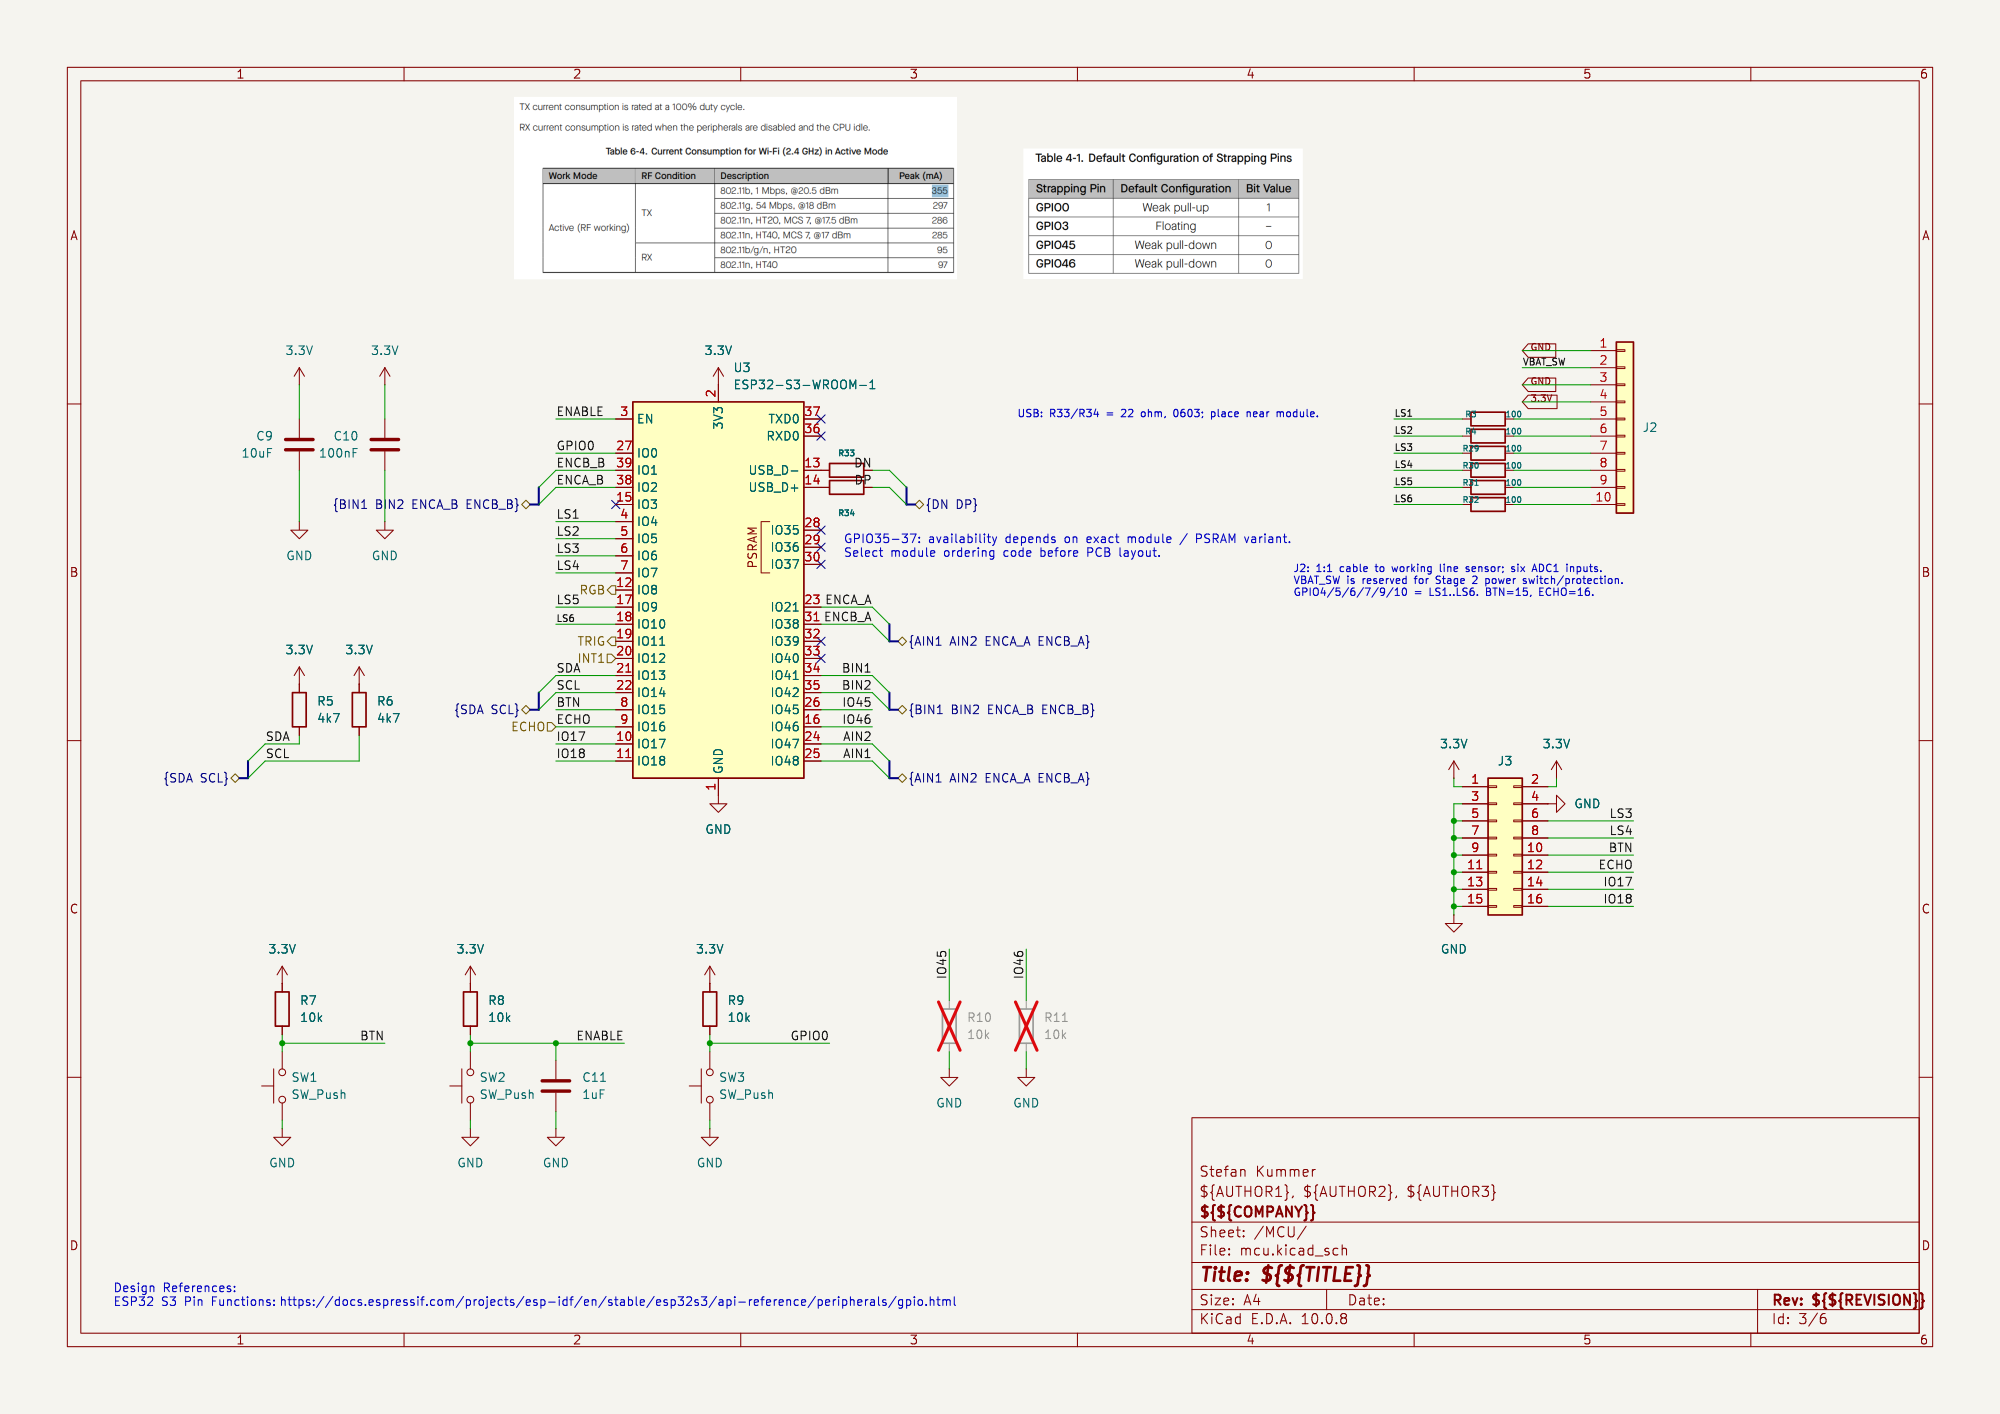
\includegraphics[width=\textwidth]{figures/pcb_main_mcu.png}
    \caption{Mikrocontroller-Schaltplan (\texttt{ESP32-S3}, Busgruppen).}
    \label{fig:pcb_main_mcu}
  \end{subfigure}
  \hfill
  \begin{subfigure}[b]{0.43\textwidth}
    \centering
    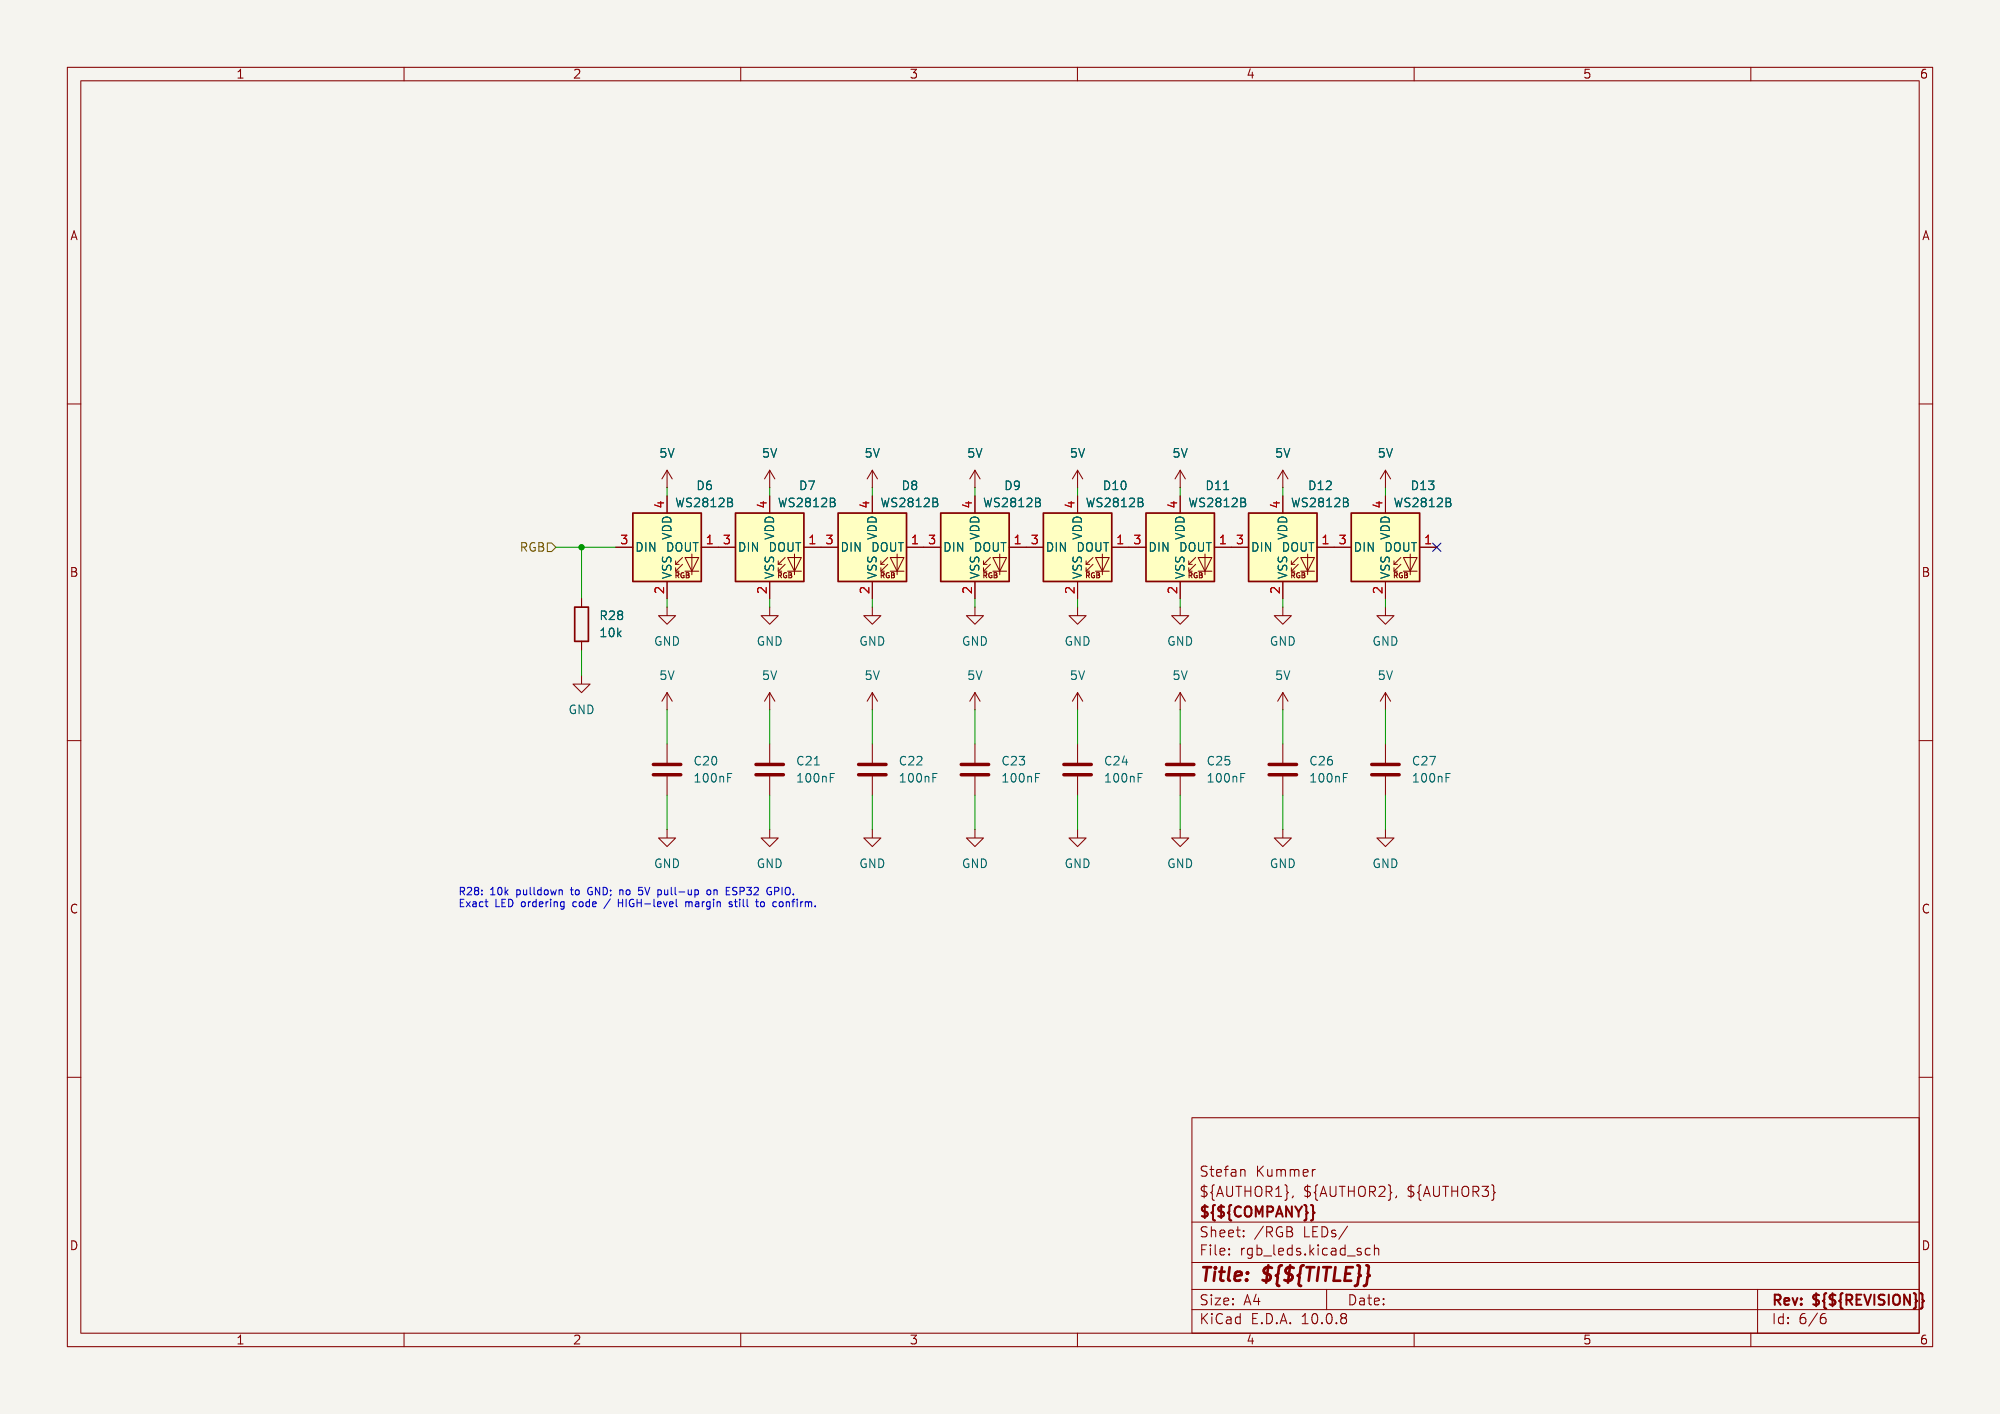
\includegraphics[width=\textwidth]{figures/pcb_main_rgb.png}
    \caption{Status-LED-Teilschaltung (\texttt{R28} Pulldown).}
    \label{fig:pcb_main_rgb}
  \end{subfigure}
  \caption{Schaltplanauszüge der Hauptplatine \texttt{Tumbler\_Stage1} (KiCad~10).}
  \label{fig:pcb_main_sch}
\end{figure}

\subsection{Übergang zu Stufe 2 und Leistungs- bzw. Akkulaufzeitbilanz}
\label{sec:leistungsbilanz}
Die gezielte Netzlistenprüfung von \texttt{Tumbler\_Stage1} bestätigte 51 von 51 Signalverbindungen ohne Befund (ERC-Kategorien \texttt{net\_not\_bus\_member}, \texttt{pin\_not\_driven} und \texttt{multiple\_net\_names} jeweils~0). Im ungefilterten Gesamt-ERC verblieben lediglich drei dokumentierte Meldungen (\texttt{power\_pin\_not\_driven}, \texttt{isolated\_pin\_label} sowie \texttt{pin\_to\_pin}), die direkt auf den bewusst noch offenen Leistungspfad von \texttt{VBAT\_SW} zurückgehen. Dieser wird in Stufe~2 gemeinsam mit der 2S-USB-C-Lade- und Schutzschaltung sowie der endgültigen Entscheidung zwischen \emph{LSM6DSV} und \emph{MPU6050} geschlossen.

Für die Auslegung der Strompfade und Sicherungen wurde eine vollständige Leistungsbilanz bei Nennspannung $U_{\mathrm{Bat}} = \qty{7,4}{\volt}$ aufgestellt (Tabelle~\ref{tab:leistungsbilanz}).

\begin{table}[htbp]
\centering
\caption{Strom- und Leistungsbilanz des Tumbler~v3.0 im normalen Fahrbetrieb und im Blockierfall.}
\label{tab:leistungsbilanz}
\begin{tabular}{@{}p{4.6cm}c c c c@{}}
\toprule
\textbf{Verbraucher} & \textbf{Schiene} & \textbf{Typ. Strom} & \textbf{Max. Strom} & \textbf{Typ. Leistung} \\
\midrule
ESP32-S3-WROOM-1 (Dual-Core) & \qty{3,3}{\volt} & \qty{140}{\milli\ampere} & \qty{350}{\milli\ampere} & \qty{0,46}{\watt} \\
8$\times$ VL53L0/1XV2 (kontinuierlich) & \qty{3,3}{\volt} & \qty{160}{\milli\ampere} & \qty{240}{\milli\ampere} & \qty{0,53}{\watt} \\
6$\times$ CNY70 Phototransistoren + IMU & \qty{3,3}{\volt} & \qty{15}{\milli\ampere} & \qty{25}{\milli\ampere} & \qty{0,05}{\watt} \\
6$\times$ CNY70 IR-LEDs (2 Stränge) & \texttt{VBAT\_SW} & \qty{40}{\milli\ampere} & \qty{52}{\milli\ampere} & \qty{0,30}{\watt} \\
2$\times$ GA37-520 Motoren (Fahrt / Stall) & \texttt{VBAT\_SW} & \qty{600}{\milli\ampere} & \qty{3200}{\milli\ampere} & \qty{4,44}{\watt} \\
\midrule
\textbf{Gesamt (inkl. $\eta_{\mathrm{Buck}} = 90\,\%$)} & \textbf{2S Li-Ion} & \textbf{$\approx \qty{800}{\milli\ampere}$} & \textbf{$\approx \qty{3550}{\milli\ampere}$} & \textbf{$\approx \qty{5,9}{\watt}$} \\
\bottomrule
\end{tabular}
\end{table}

Mit einem gängigen 2S-Li-Ion-Pack der Kapazität $C_{\mathrm{Bat}} = \qty{2600}{\milli\ampere\hour}$ und einer nutzbaren Entladetiefe von \qty{85}{\percent} ergibt sich im kontinuierlichen Fahr- und Einparkbetrieb eine rechnerische Betriebsdauer von:
\begin{equation}
  t_{\mathrm{Betrieb}} \approx \frac{0{,}85 \cdot \qty{2600}{\milli\ampere\hour}}{\qty{800}{\milli\ampere}} \approx \qty{2,76}{\hour}
  \label{eq:akkulaufzeit}
\end{equation}
Damit ist ein ganzer Labor- oder Prüfungstag problemlos mit einer einzigen Akkuladung abdeckbar.

% ==============================================================================
\section{Mechanische Konstruktion und CAD-Evolution (v1 bis v10.0)}
\label{sec:cad_evolution}
% ==============================================================================
Das Fahrgestell bildet das mechanische Rückgrat des Roboters. Statt einer manuellen, schwer änderbaren Maus-Konstruktion wurde das komplette Chassis samt einem 127-Körper-Digital-Mock-Up (\gls{dmu}) parametrisch in Python (\texttt{build123d} / OpenCASCADE BRep-Kern sowie Fusion-360-API-Skripte) nach dem \gls{ssot}-Prinzip aufgebaut. Jede Änderung an Platinenmaßen, Schraubenabständen oder Wandstärken propagiert dadurch automatisch und widerspruchsfrei in das gesamte 3D-Modell.

\subsection{Chronologische Fehleranalyse und Iterationsstufen}
Die Entwicklung durchlief zehn konstruktive Hauptrevisionen, in denen reale Probleme aus der Vorversion schrittweise aufgedeckt und systematisch beseitigt wurden (Tabelle~\ref{tab:cad_evolution}).

\begin{table}[htbp]
\centering
\caption{Entwicklungshistorie des 3D-Chassis von der Nachkonstruktion (v1) bis zum druckfertigen Release (v10.0).}
\label{tab:cad_evolution}
\begin{tabular}{@{}p{1.5cm}p{3.6cm}p{8.9cm}@{}}
\toprule
\textbf{Version} & \textbf{Schwerpunkt} & \textbf{Erkannte Schwachstelle und konstruktive Lösung} \\
\midrule
v1--v2 & Reverse Engineering & Nachbildung des handvermessenen Originalgehäuses (\qtyproduct{120 x 176}{\milli\meter}). Ergebnis: zu wenig Bauraum für 2S-Akku und keine geschützten LiDAR-Aufnahmen. \\
v3 & Integration 6$\times$ LiDAR & Erste integrierte Sensor-Pods für \emph{VL53L0/1XV2} (\qty{19,5}{\milli\meter} Lochabstand). Schwachstelle: zu wenig Platz hinter verlöteten Stiftleisten zum Einstecken von Dupont-Kabeln. \\
v4--v6 & Crash-Bumper \& Stecker-Dummies & Einführung eines \qty{6,0}{\milli\meter} Crash-Bumpers, \qty{4,0}{\milli\meter} Bodenplatte und realer \qty{24}{\milli\meter} roter Stecker-Dummies. Erste automatisierte BRep-Kollisionsprüfung. \\
v7--v8 & Upgrade auf 8$\times$ LiDAR & Erweiterung auf \qty{360}{\degree}-Abdeckung (zusätzliche Front- und Heck-Mittensensoren \texttt{3a}/\texttt{3h}). Akkufach auf \qtyproduct{78,0 x 43,3 x 21,5}{\milli\meter} erweitert. \\
v9 & Zero-Collision-DMU & Beseitigung aller `.solids()[0]`-Trunkierungen (121 Einzelkörper geprüft), Schutz der 4 Standoffs (\texttt{H1}--\texttt{H4}) und geschlossene \qtyrange{3,85}{4,30}{\milli\meter} Pod-Dächer. \\
\textbf{v10.0} & \textbf{Print-Ready DfAM} & \textbf{1)} Blockierende Querwand hinter Motoren ($Y = +2{,}5..+4{,}5\text{ mm}$) komplett entfernt; \textbf{2)} nach oben offener \emph{Slide-In} Schalter-C-Kanal + Snap-On Clip; \textbf{3)} Stadium-Laschentaschen \& \qty{1,80}{\milli\meter} M2-Teardrop-Sacklöcher; \textbf{4)} 4$\times$ M3-Sechskant-Mutterntaschen; \textbf{5)} 100\,\% Watertight STL. \\
\bottomrule
\end{tabular}
\end{table}

Abbildung~\ref{fig:cad_evolution_imgs} illustriert diesen schrittweisen Reifeprozess vom schlichten Ausgangsmodell~(v2) über die erste LiDAR-Integration~(v3) bis zum vollständigen 127-Körper-DMU der Revision~v10.0.

\begin{figure}[htbp]
  \centering
  \begin{subfigure}[b]{0.48\textwidth}
    \centering
    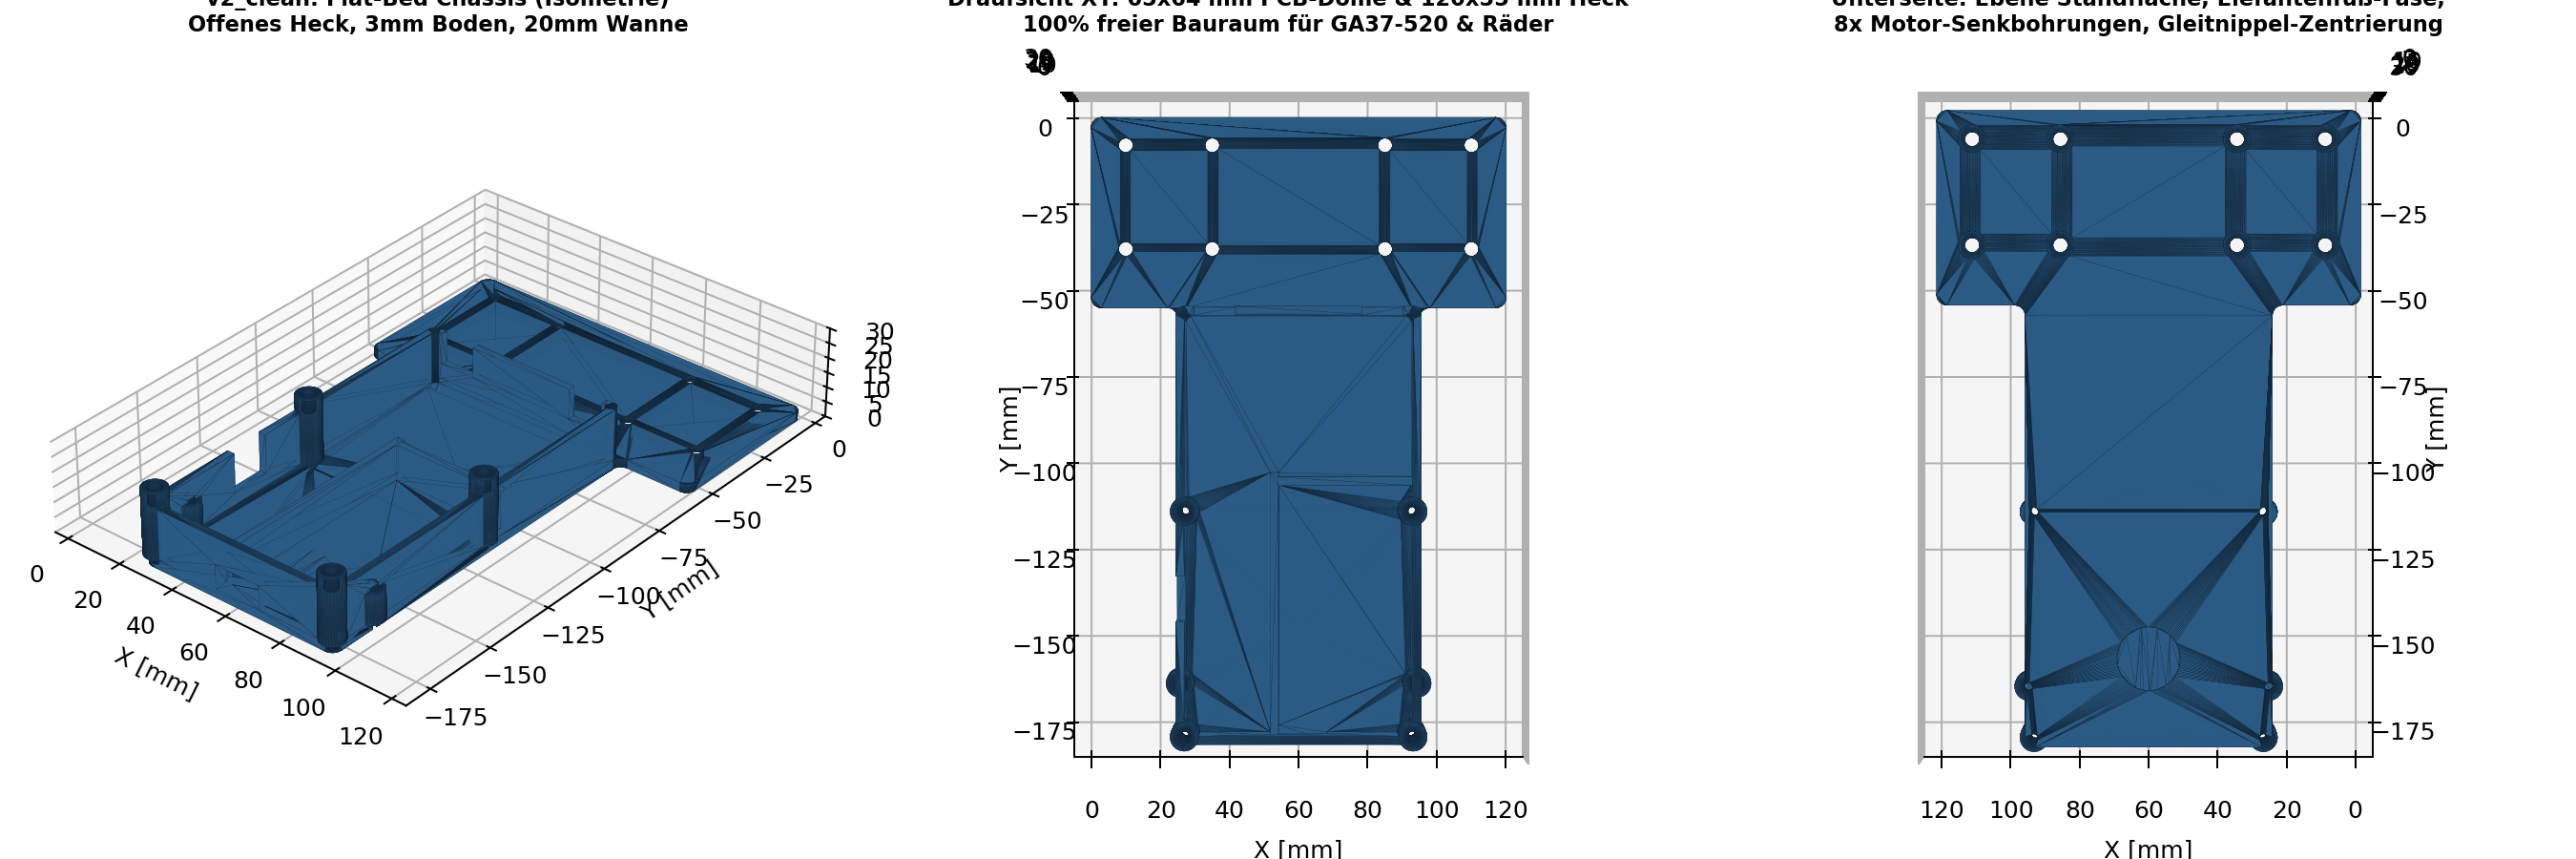
\includegraphics[width=\textwidth]{figures/v2_clean_engineering_views.png}
    \caption{Revision~v2: Nachkonstruktion des Ausgangsgehäuses.}
    \label{fig:cad_v2}
  \end{subfigure}
  \hfill
  \begin{subfigure}[b]{0.48\textwidth}
    \centering
    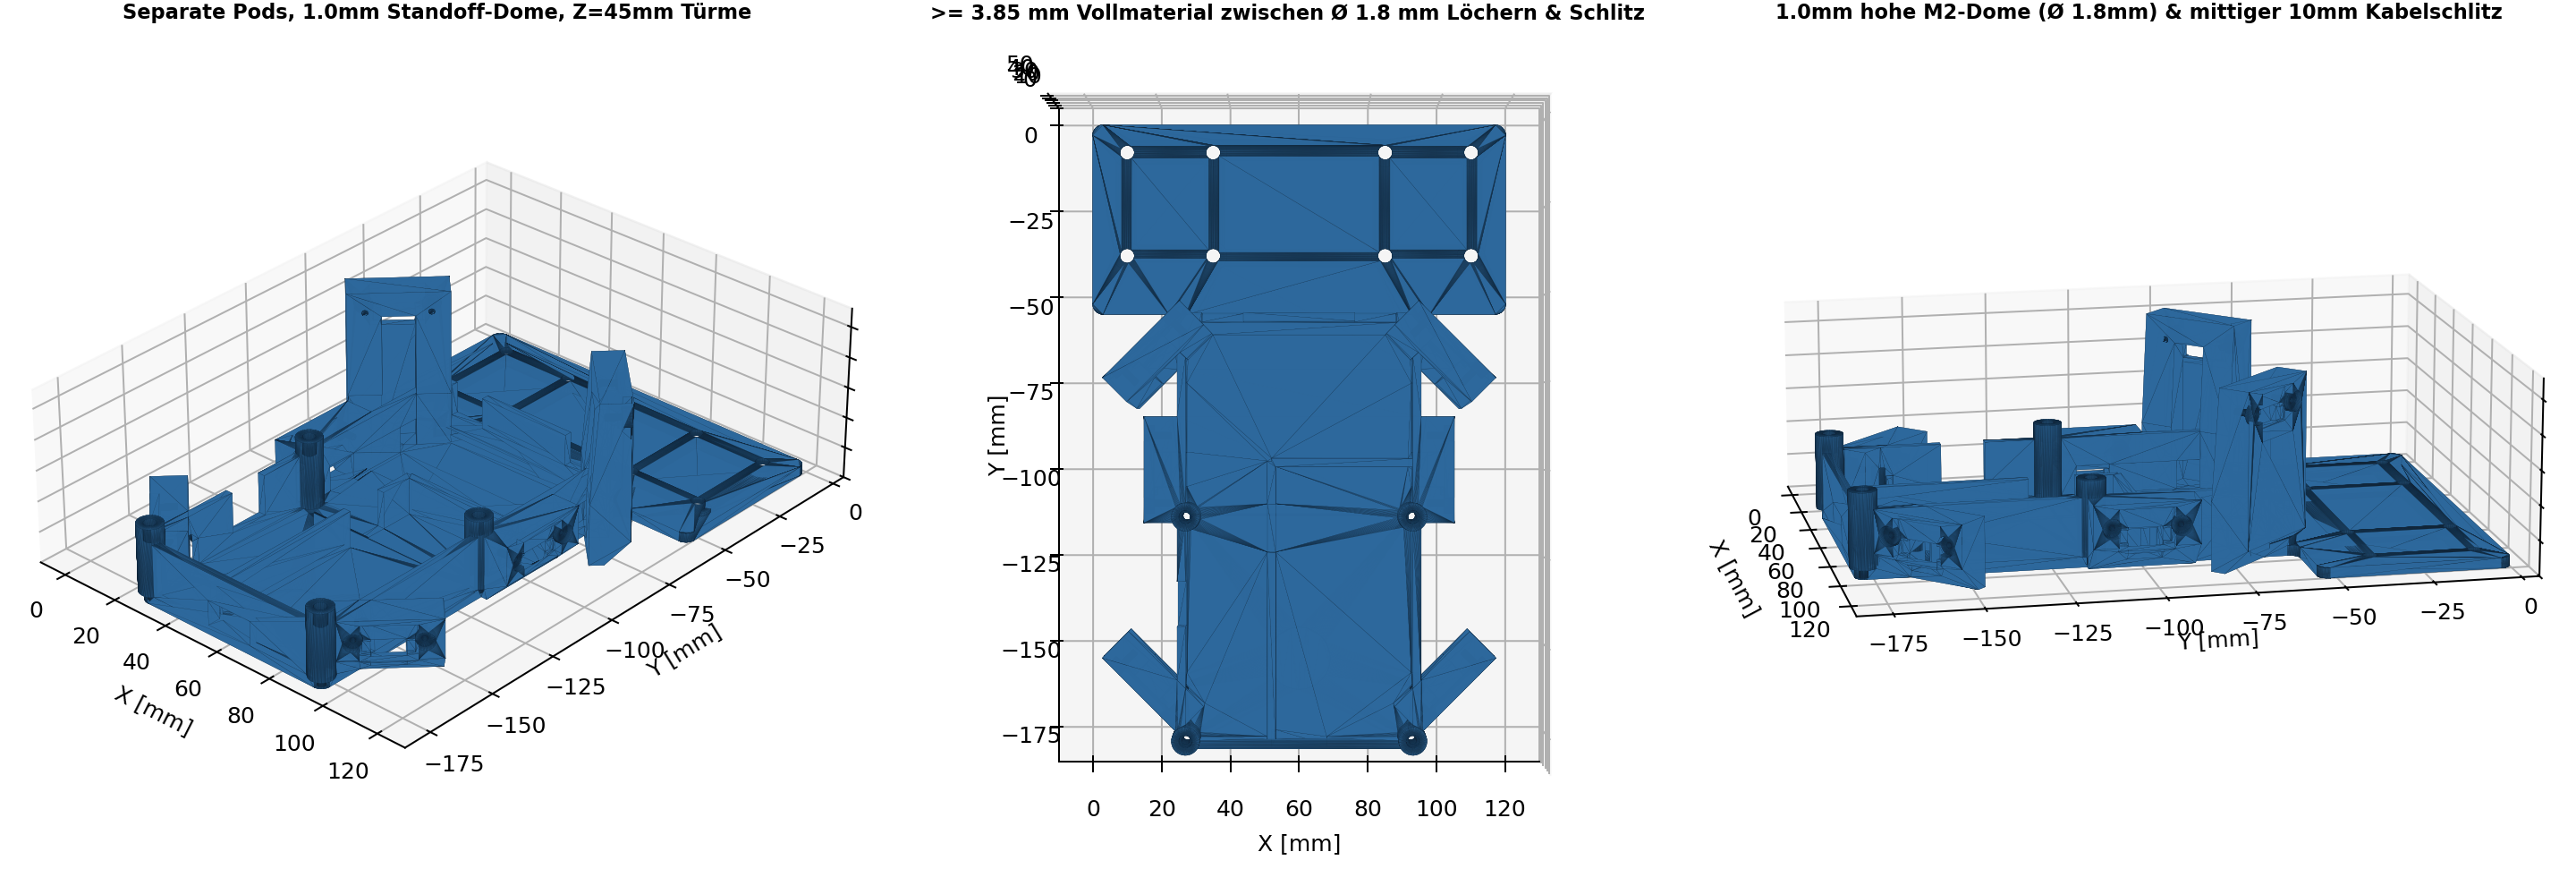
\includegraphics[width=\textwidth]{figures/v3_LiDar_V2_engineering_views.png}
    \caption{Revision~v3: Erste 6-fach-LiDAR-Integration mit Türmen.}
    \label{fig:cad_v3}
  \end{subfigure}
  \vspace{0.4cm}
  \begin{subfigure}[b]{0.98\textwidth}
    \centering
    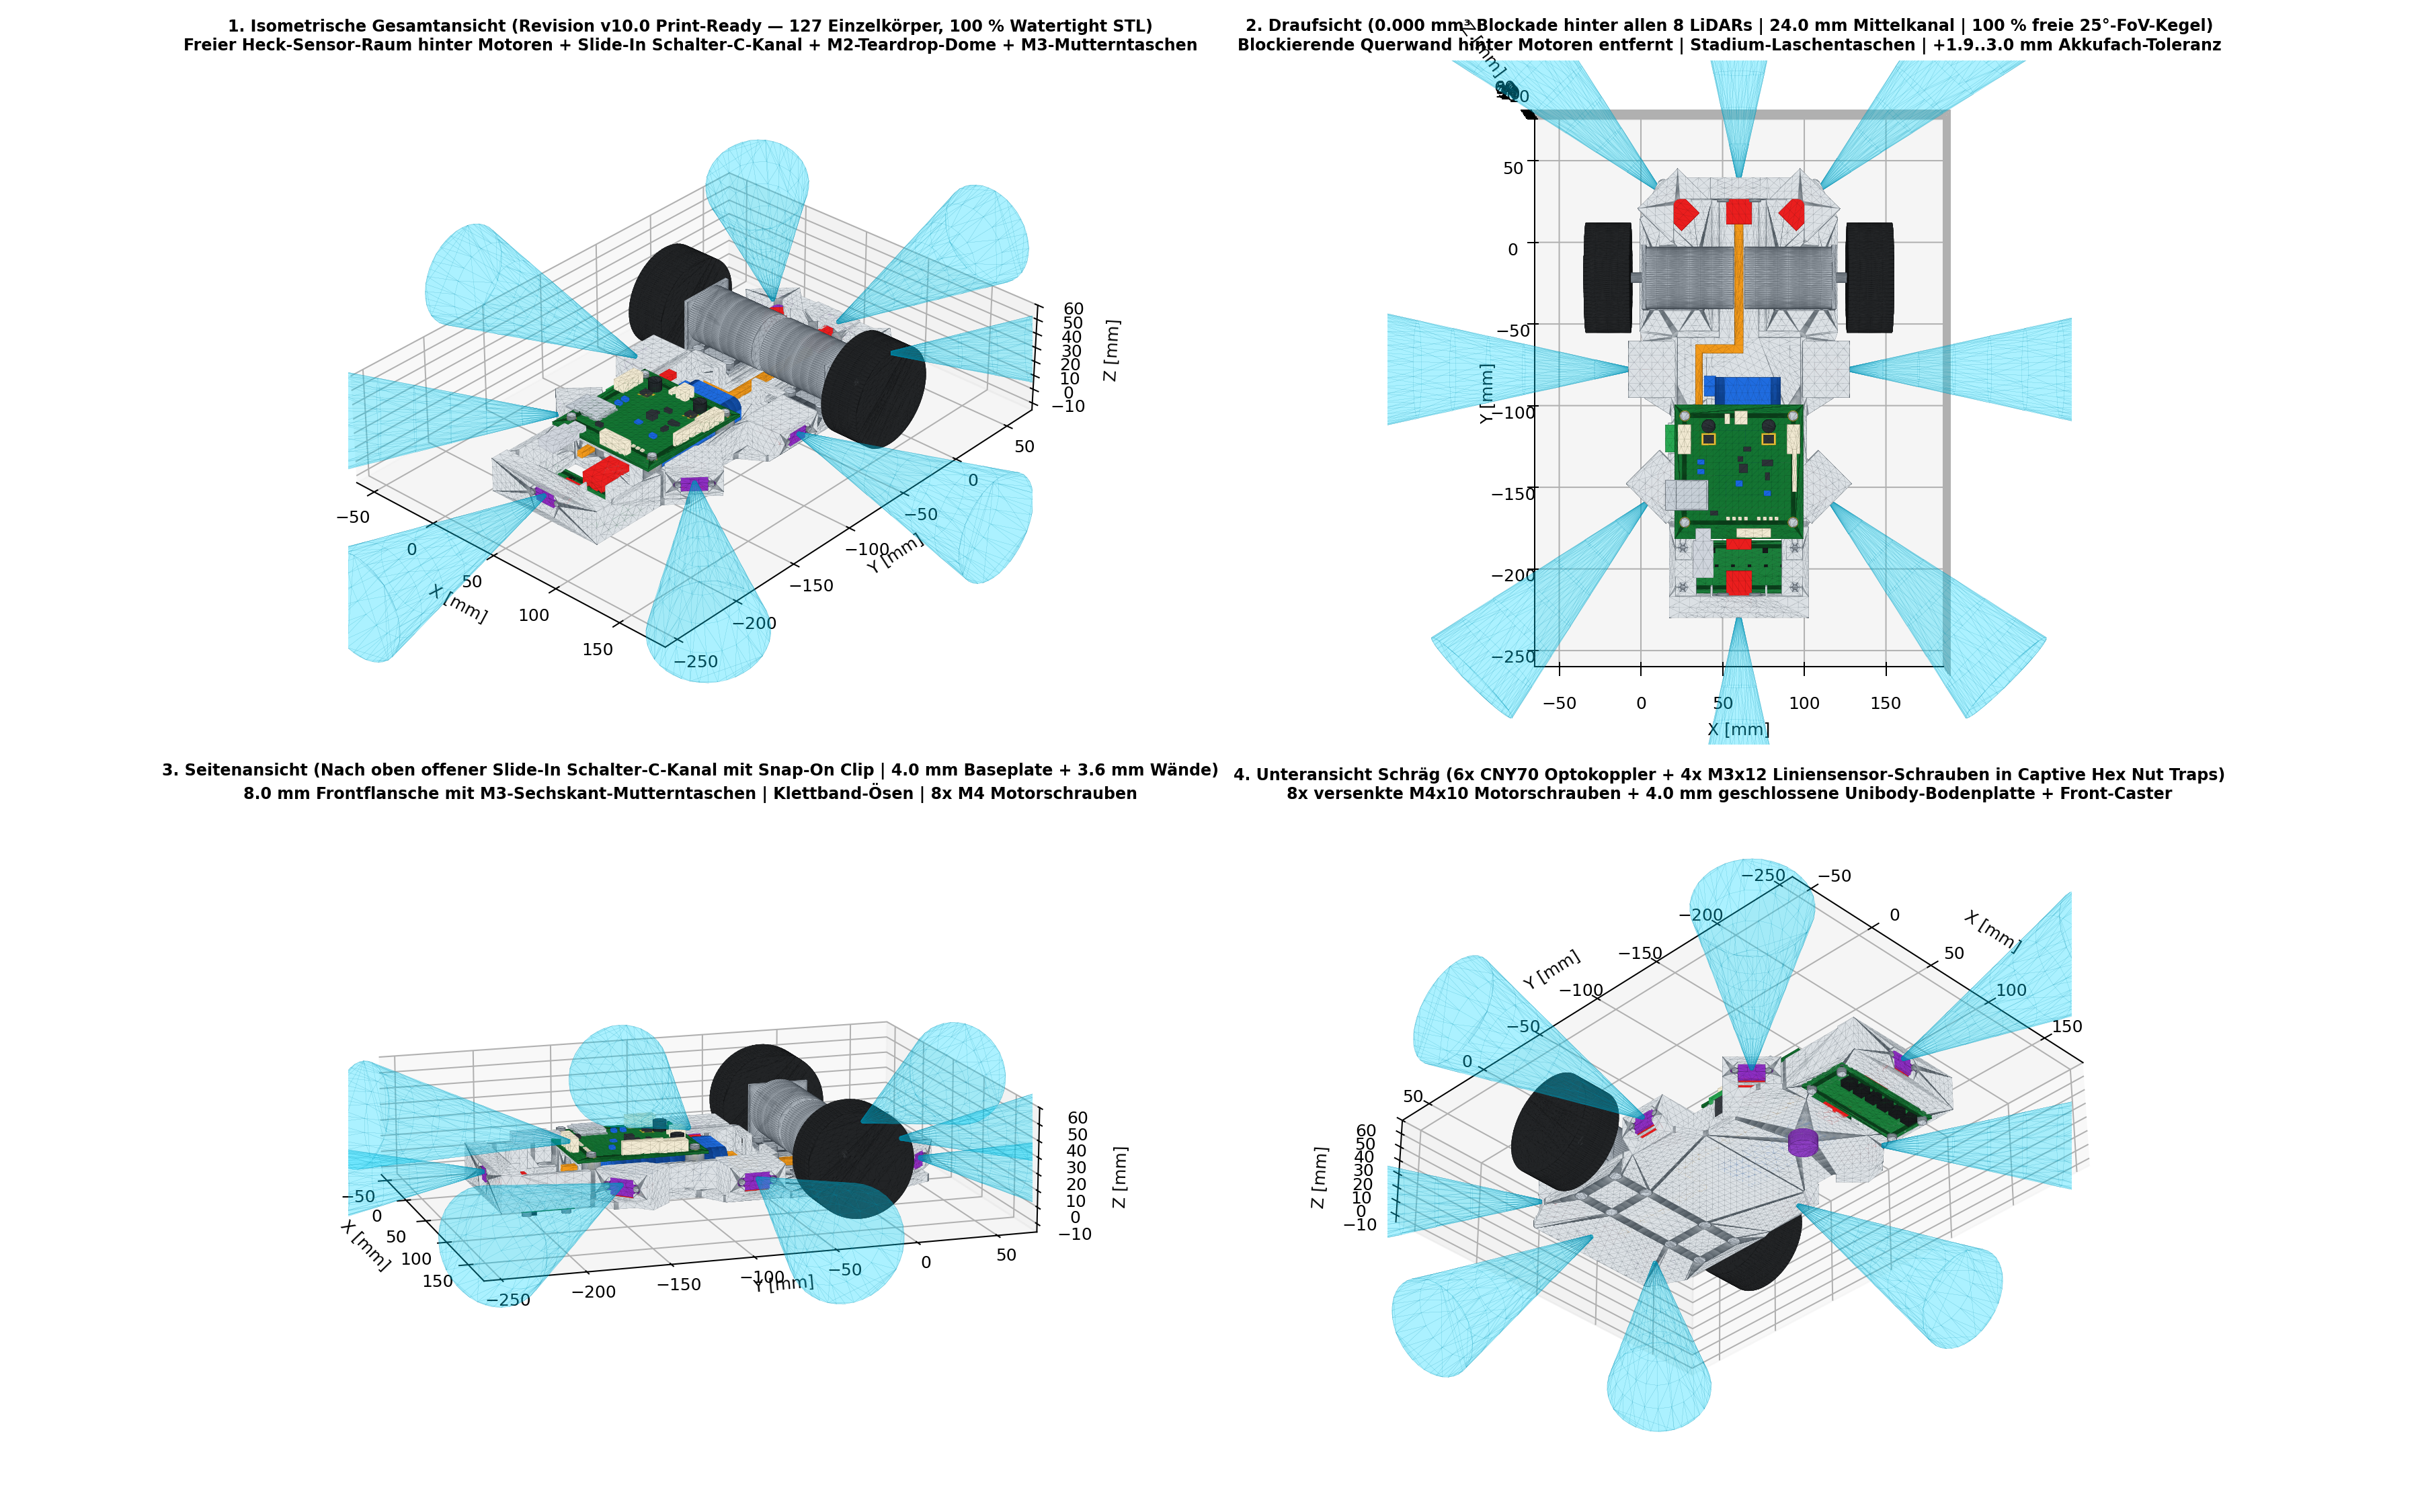
\includegraphics[width=\textwidth]{figures/cad_v10_master_dmu.png}
    \caption{Revision~v10.0 (Print-Ready): Vollständiges 127-Körper-DMU mit 8$\times$ \qty{25}{\degree}-FoV-Sichtkegeln, allen SMD-Bauteilen, 24-mm-Stecker-Dummies, Schrauben und 3D-Kabelbaum (\qty{0,000}{\milli\meter\cubed} Kollision).}
    \label{fig:cad_v10_master}
  \end{subfigure}
  \caption{Evolution des 3D-Chassis vom Grundkörper~(v2) bis zum fertigungsreifen Digital Mock-Up~(v10.0).}
  \label{fig:cad_evolution_imgs}
\end{figure}

\begin{figure}[htbp]
  \centering
  \begin{subfigure}[b]{0.48\textwidth}
    \centering
    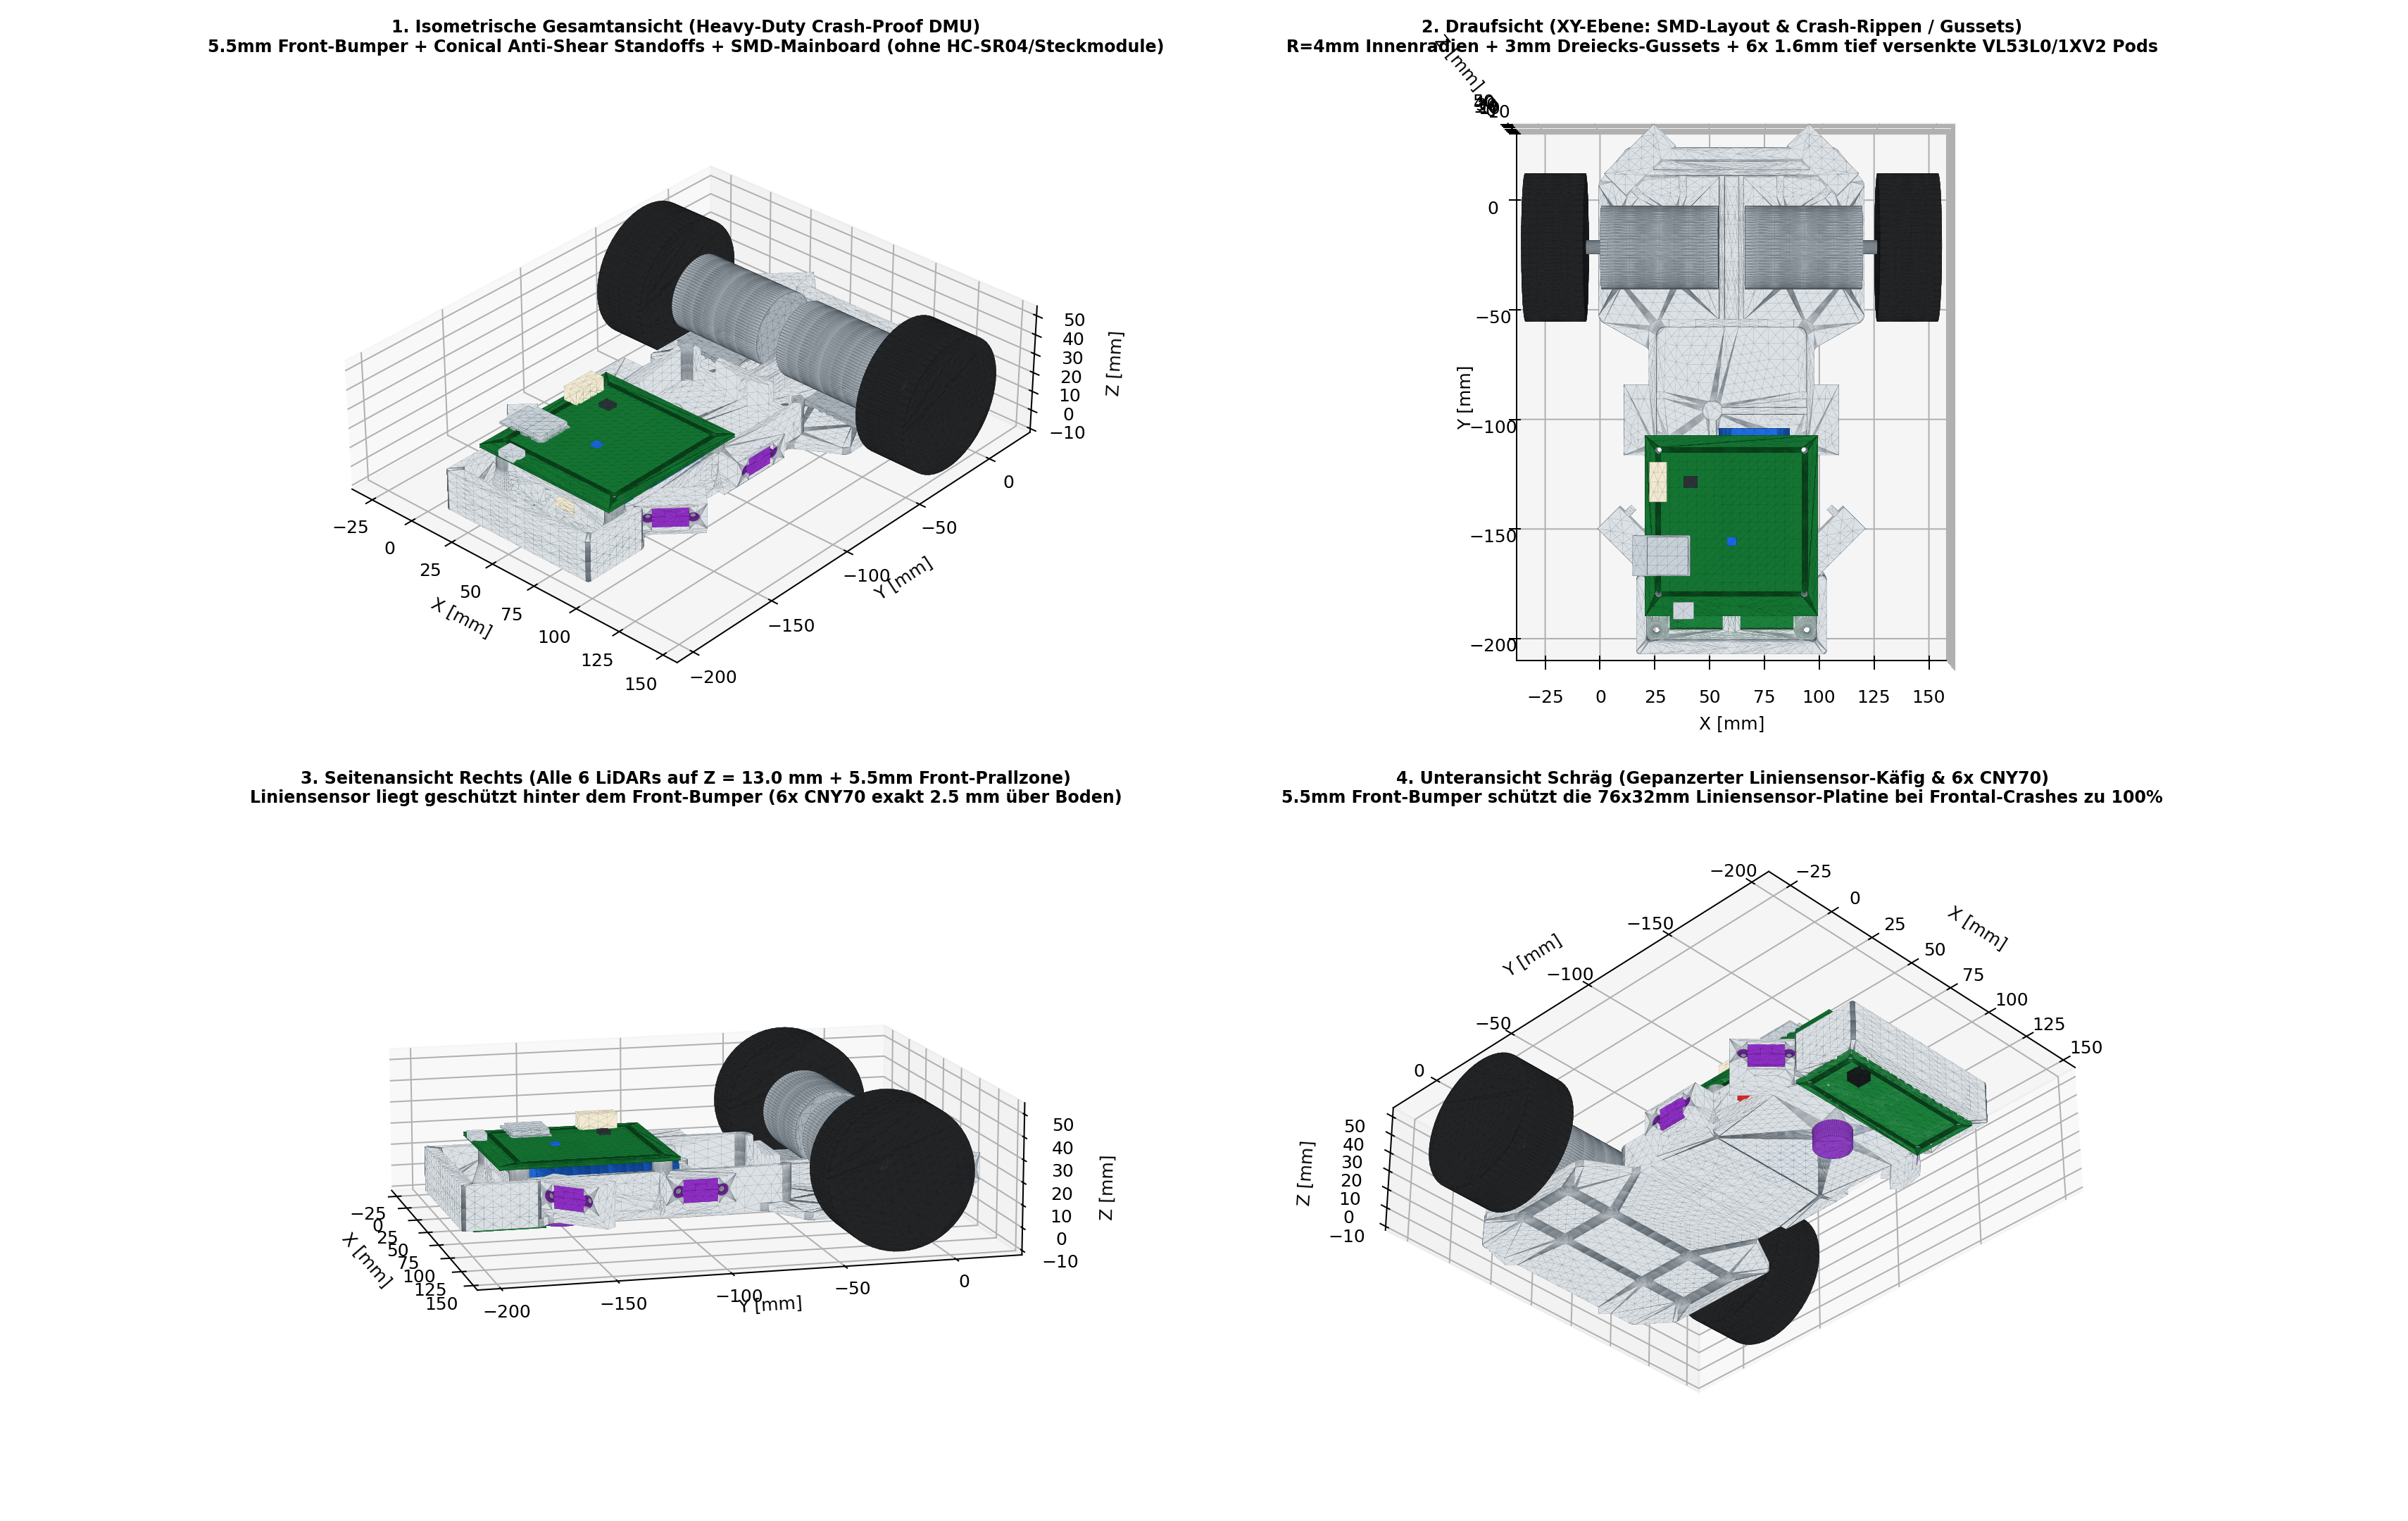
\includegraphics[width=\textwidth]{figures/cad_v4_crashproof.png}
    \caption{Revision~v4: Einführung des 6-mm-Crash-Bumpers und roter 24-mm-Stecker-Dummies.}
    \label{fig:cad_v4}
  \end{subfigure}
  \hfill
  \begin{subfigure}[b]{0.48\textwidth}
    \centering
    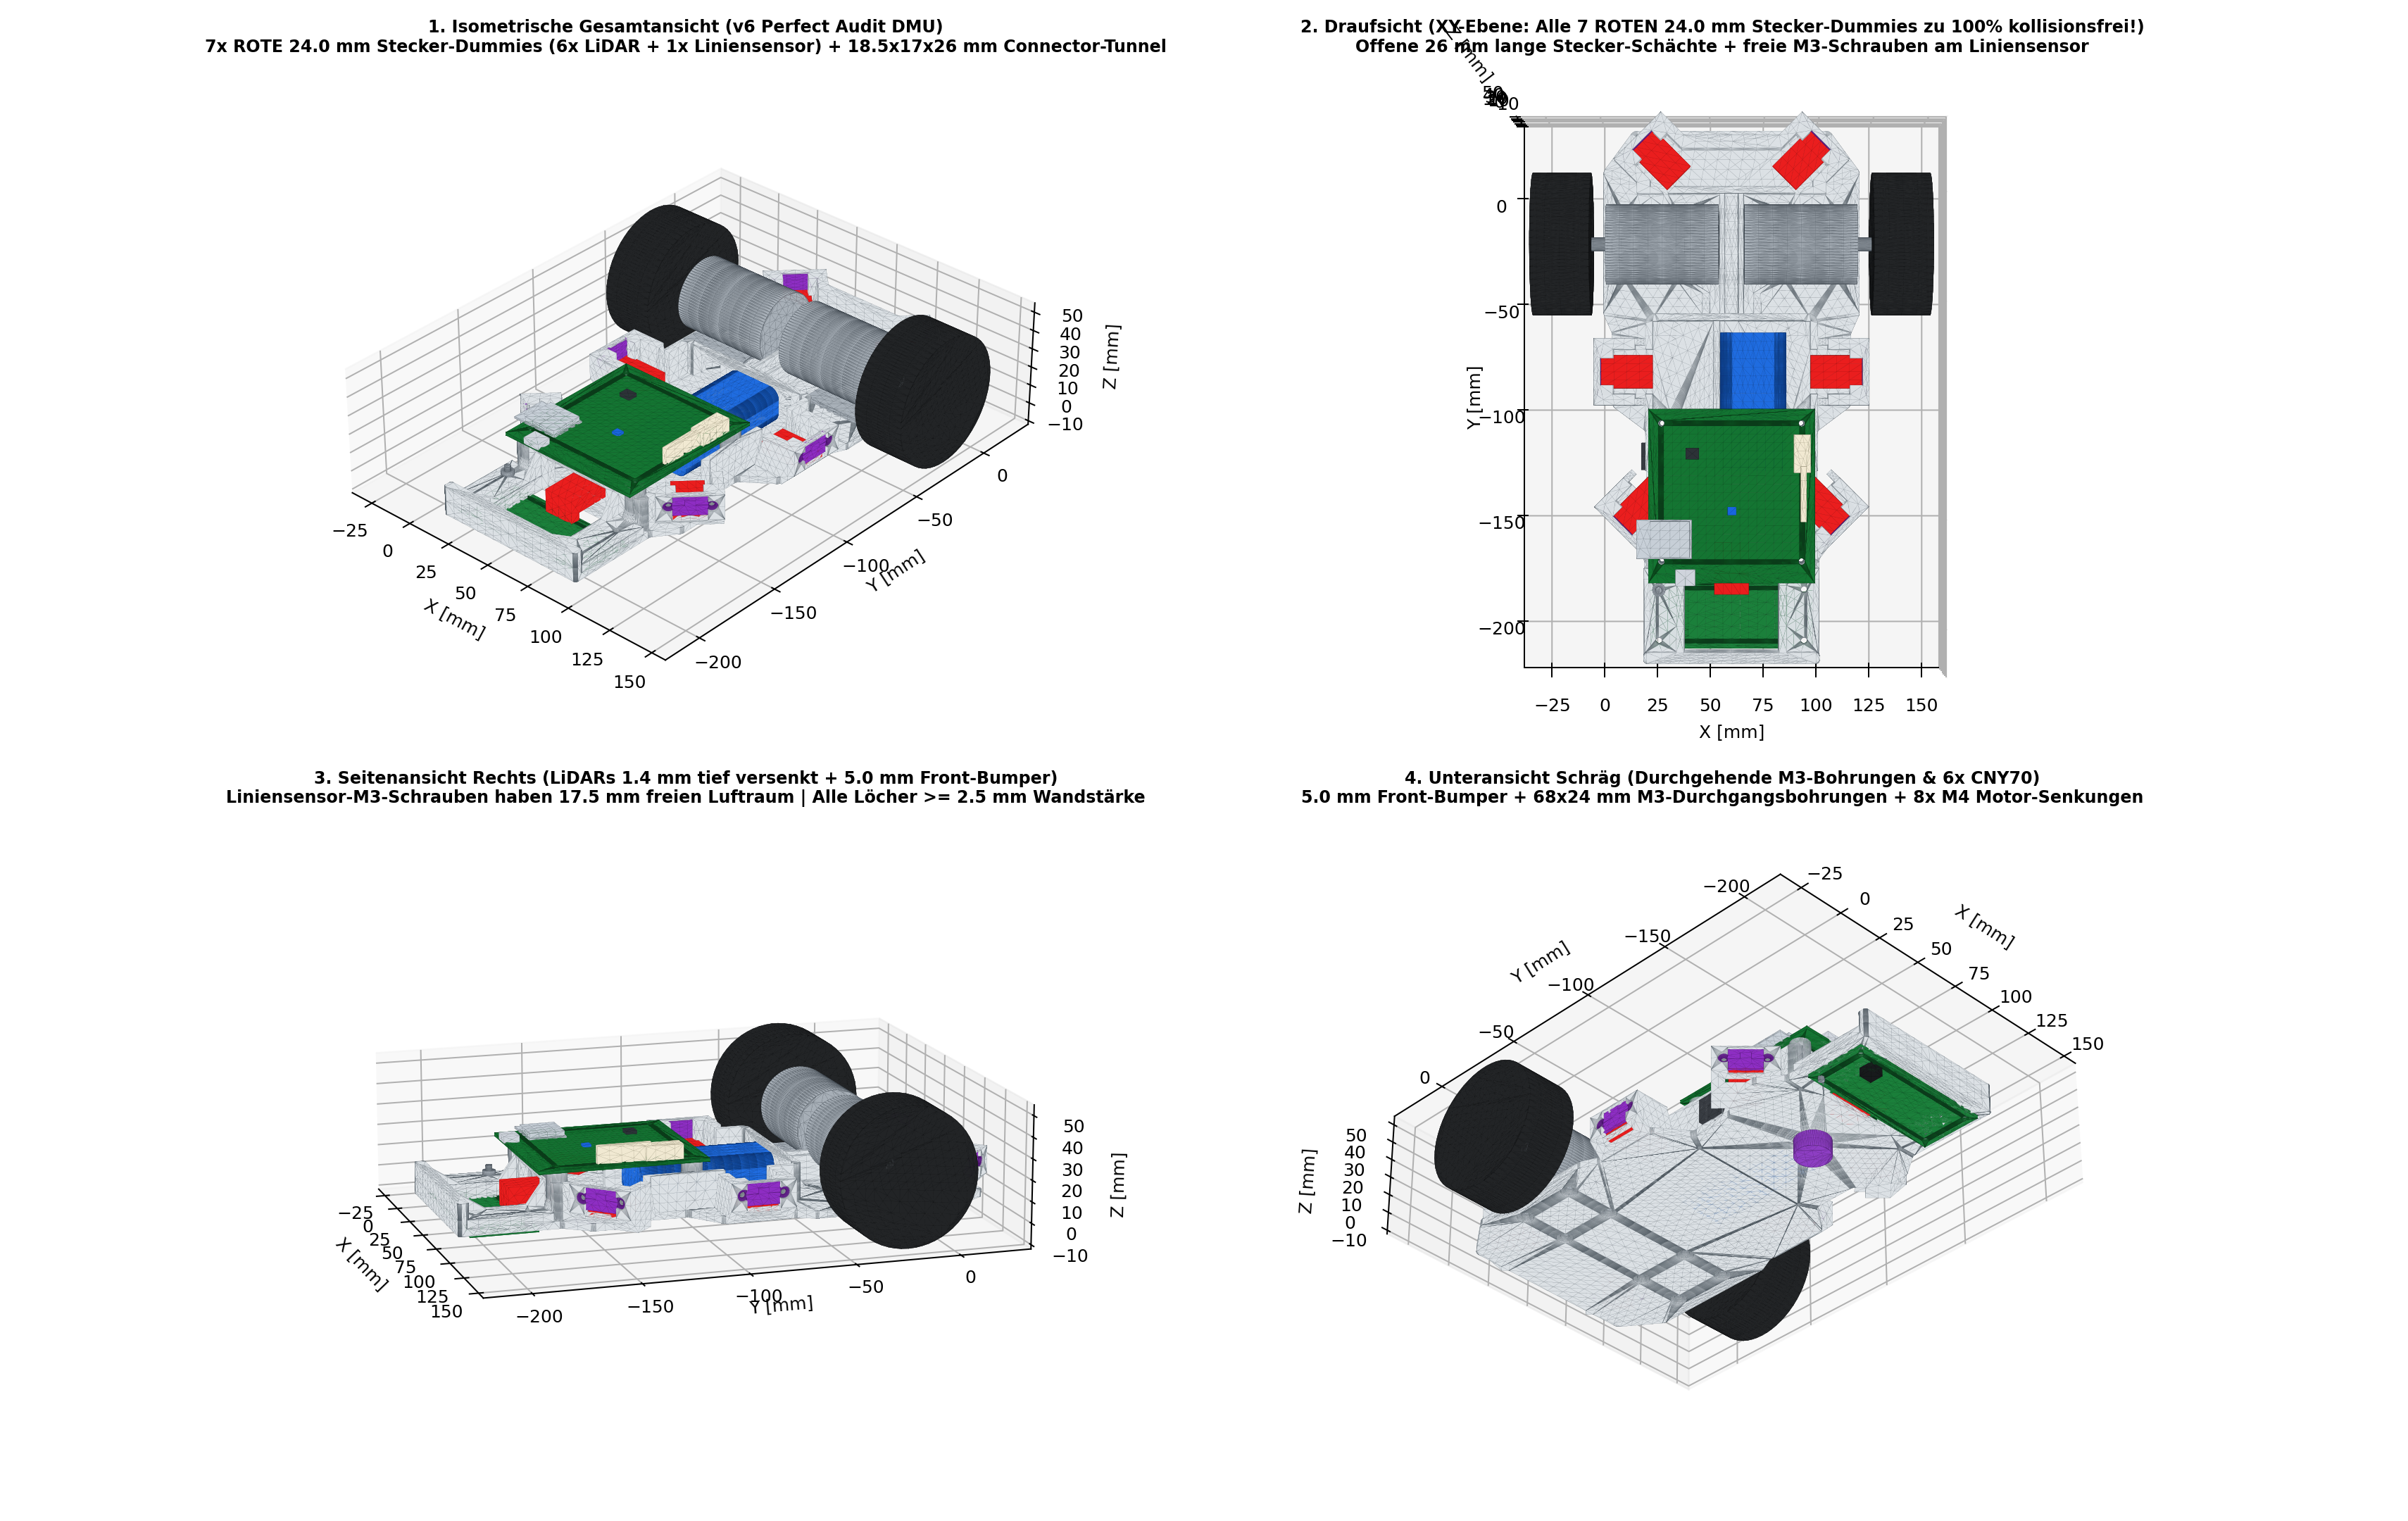
\includegraphics[width=\textwidth]{figures/cad_v6_audit.png}
    \caption{Revision~v6: Erster vollständiger 6-Sensor-BRep-Kollisions-Audit.}
    \label{fig:cad_v6}
  \end{subfigure}
  \caption{Zwischenstufen v4 und v6 der parametrischen CAD-Entwicklung vor dem Upgrade auf 8$\times$ LiDAR.}
  \label{fig:cad_v4_v6}
\end{figure}

\subsection{Detailkonstruktion der kritischen Baugruppen in Revision v10.0}
Bei der abschließenden Vor-Druck-Prüfung von Revision~v9 anhand von Horizontalschnitten fielen drei praxisrelevante Montagehindernisse auf, die erst in Revision~v10.0 vollständig behoben wurden (siehe Detail-Zooms in Abbildung~\ref{fig:cad_v10_zooms} sowie die sechs Horizontalschnitte in Abbildung~\ref{fig:cad_v10_slices}):

\begin{enumerate}
  \item \textbf{Freiräumung des Heck-Sensorbereichs hinter den Motoren:} In Revision~v9 bildete die Vorderkante des hinteren Stoßfängers zwischen $Y = \qty{+2,5}{\milli\meter}$ und $Y = \qty{+4,5}{\milli\meter}$ eine durchgehende \qty{2,0}{\milli\meter} starke Querwand über die gesamte Fahrzeugbreite. Dadurch waren die rückwärtigen Steckerzugänge der Sensoren \texttt{3f}, \texttt{3g} und \texttt{3h} vom Motorraum abgetrennt; zusätzlich ragten die äußeren Bumper-Ecken um \qty{30,49}{\milli\meter\cubed} vor die seitlichen Befestigungslaschen von \texttt{3f} und \texttt{3g}. In v10.0 wurde diese Querwand ersatzlos entfernt: Der offene Servicebereich (\texttt{rear\_plaza}) erstreckt sich nun von $Y = \qty{-4,0}{\milli\meter}$ bis $Y = \qty{+24,8}{\milli\meter}$ über die volle Breite $X = \qtyrange{20,5}{99,5}{\milli\meter}$ und mündet direkt in einen \qty{24,0}{\milli\meter} breiten Mittelkanal ($X = \qtyrange{48}{72}{\milli\meter}$). Zwei durchgehende Längs-Versteifungsrippen ($Z = \qtyrange{4,0}{6,8}{\milli\meter}$) verlaufen mit \qty{0,5}{\milli\meter} Luft unterhalb der \emph{GA37-520}-Motoren ($Z \ge \qty{7,3}{\milli\meter}$) und stellen die volle Biegesteifigkeit des Hecks sicher.
  \item \textbf{Nach oben offener „Slide-In“-C-Führungskanal für den Ein-/Aus-Schalter:} Da der \qtyproduct{13 x 13}{\milli\meter} große Wippenschalter vor dem Einbau bereits fest mit den Akkuzuleitungen verlötet ist, blockierte ein geschlossener oberer Wandriegel das Einschieben. In v10.0 ist die linke Seitenwand bei $Y = \qtyrange{-128,15}{-114,85}{\milli\meter}$ ab $Z = \qty{8,35}{\milli\meter}$ nach oben vollständig geöffnet. Ein gestuftes C-Profil (\qty{15,2}{\milli\meter} äußere Blendennut, \qty{13,3}{\milli\meter} Körperführung, \qty{10,2}{\milli\meter} innerer Lötfahnenschlitz) mit \qty{45}{\degree}-Einführfase hält den Schalter beim Betätigen formschlüssig in $+X$- und $-X$-Richtung fest. Ein separat druckbarer, werkzeugloser \emph{Snap-On}-Halteclip (\texttt{5b}) verriegelt ihn abschließend nach oben.
  \item \textbf{Stadium-Laschentaschen und M2-Teardrop-Sacklöcher:} Eine genaue Analyse zeigte, dass kreisförmige Laschen-Aussparungen (\diameter\,\qty{5,9}{\milli\meter}) am Übergang zum Rechteckkörper eine Engstelle von nur \qty{4,89}{\milli\meter} erzeugen, während reale \emph{VL53L0/1XV2}-Platinen durchgehend \qty{5,50}{\milli\meter} hohe gerade Befestigungslaschen besitzen. Alle acht Taschen wurden daher als echte Stadium-/Langloch-Kontur (\qtyproduct{19,5 x 6,0}{\milli\meter} + \qtyproduct{16,3 x 11,0}{\milli\meter}) konstruiert. Die sechzehn massiven \diameter\,\qty{7,0}{\milli\meter} Schraubendome erhalten \qty{7,0}{\milli\meter} tiefe \diameter\,\qty{1,80}{\milli\meter} M2-Kernlöcher (echter \qty{0,20}{\milli\meter} Gewindebiss für selbstfurchende M2-Schrauben in PLA/PETG) mit \qty{45}{\degree}-Teardrop-First gegen Durchhängen im horizontalen FDM-Druck, \diameter\,\qty{2,2}{\milli\meter} Einführfase und \qty{3,50}{\milli\meter} geschlossenem Boden.
\end{enumerate}

\begin{figure}[htbp]
  \centering
  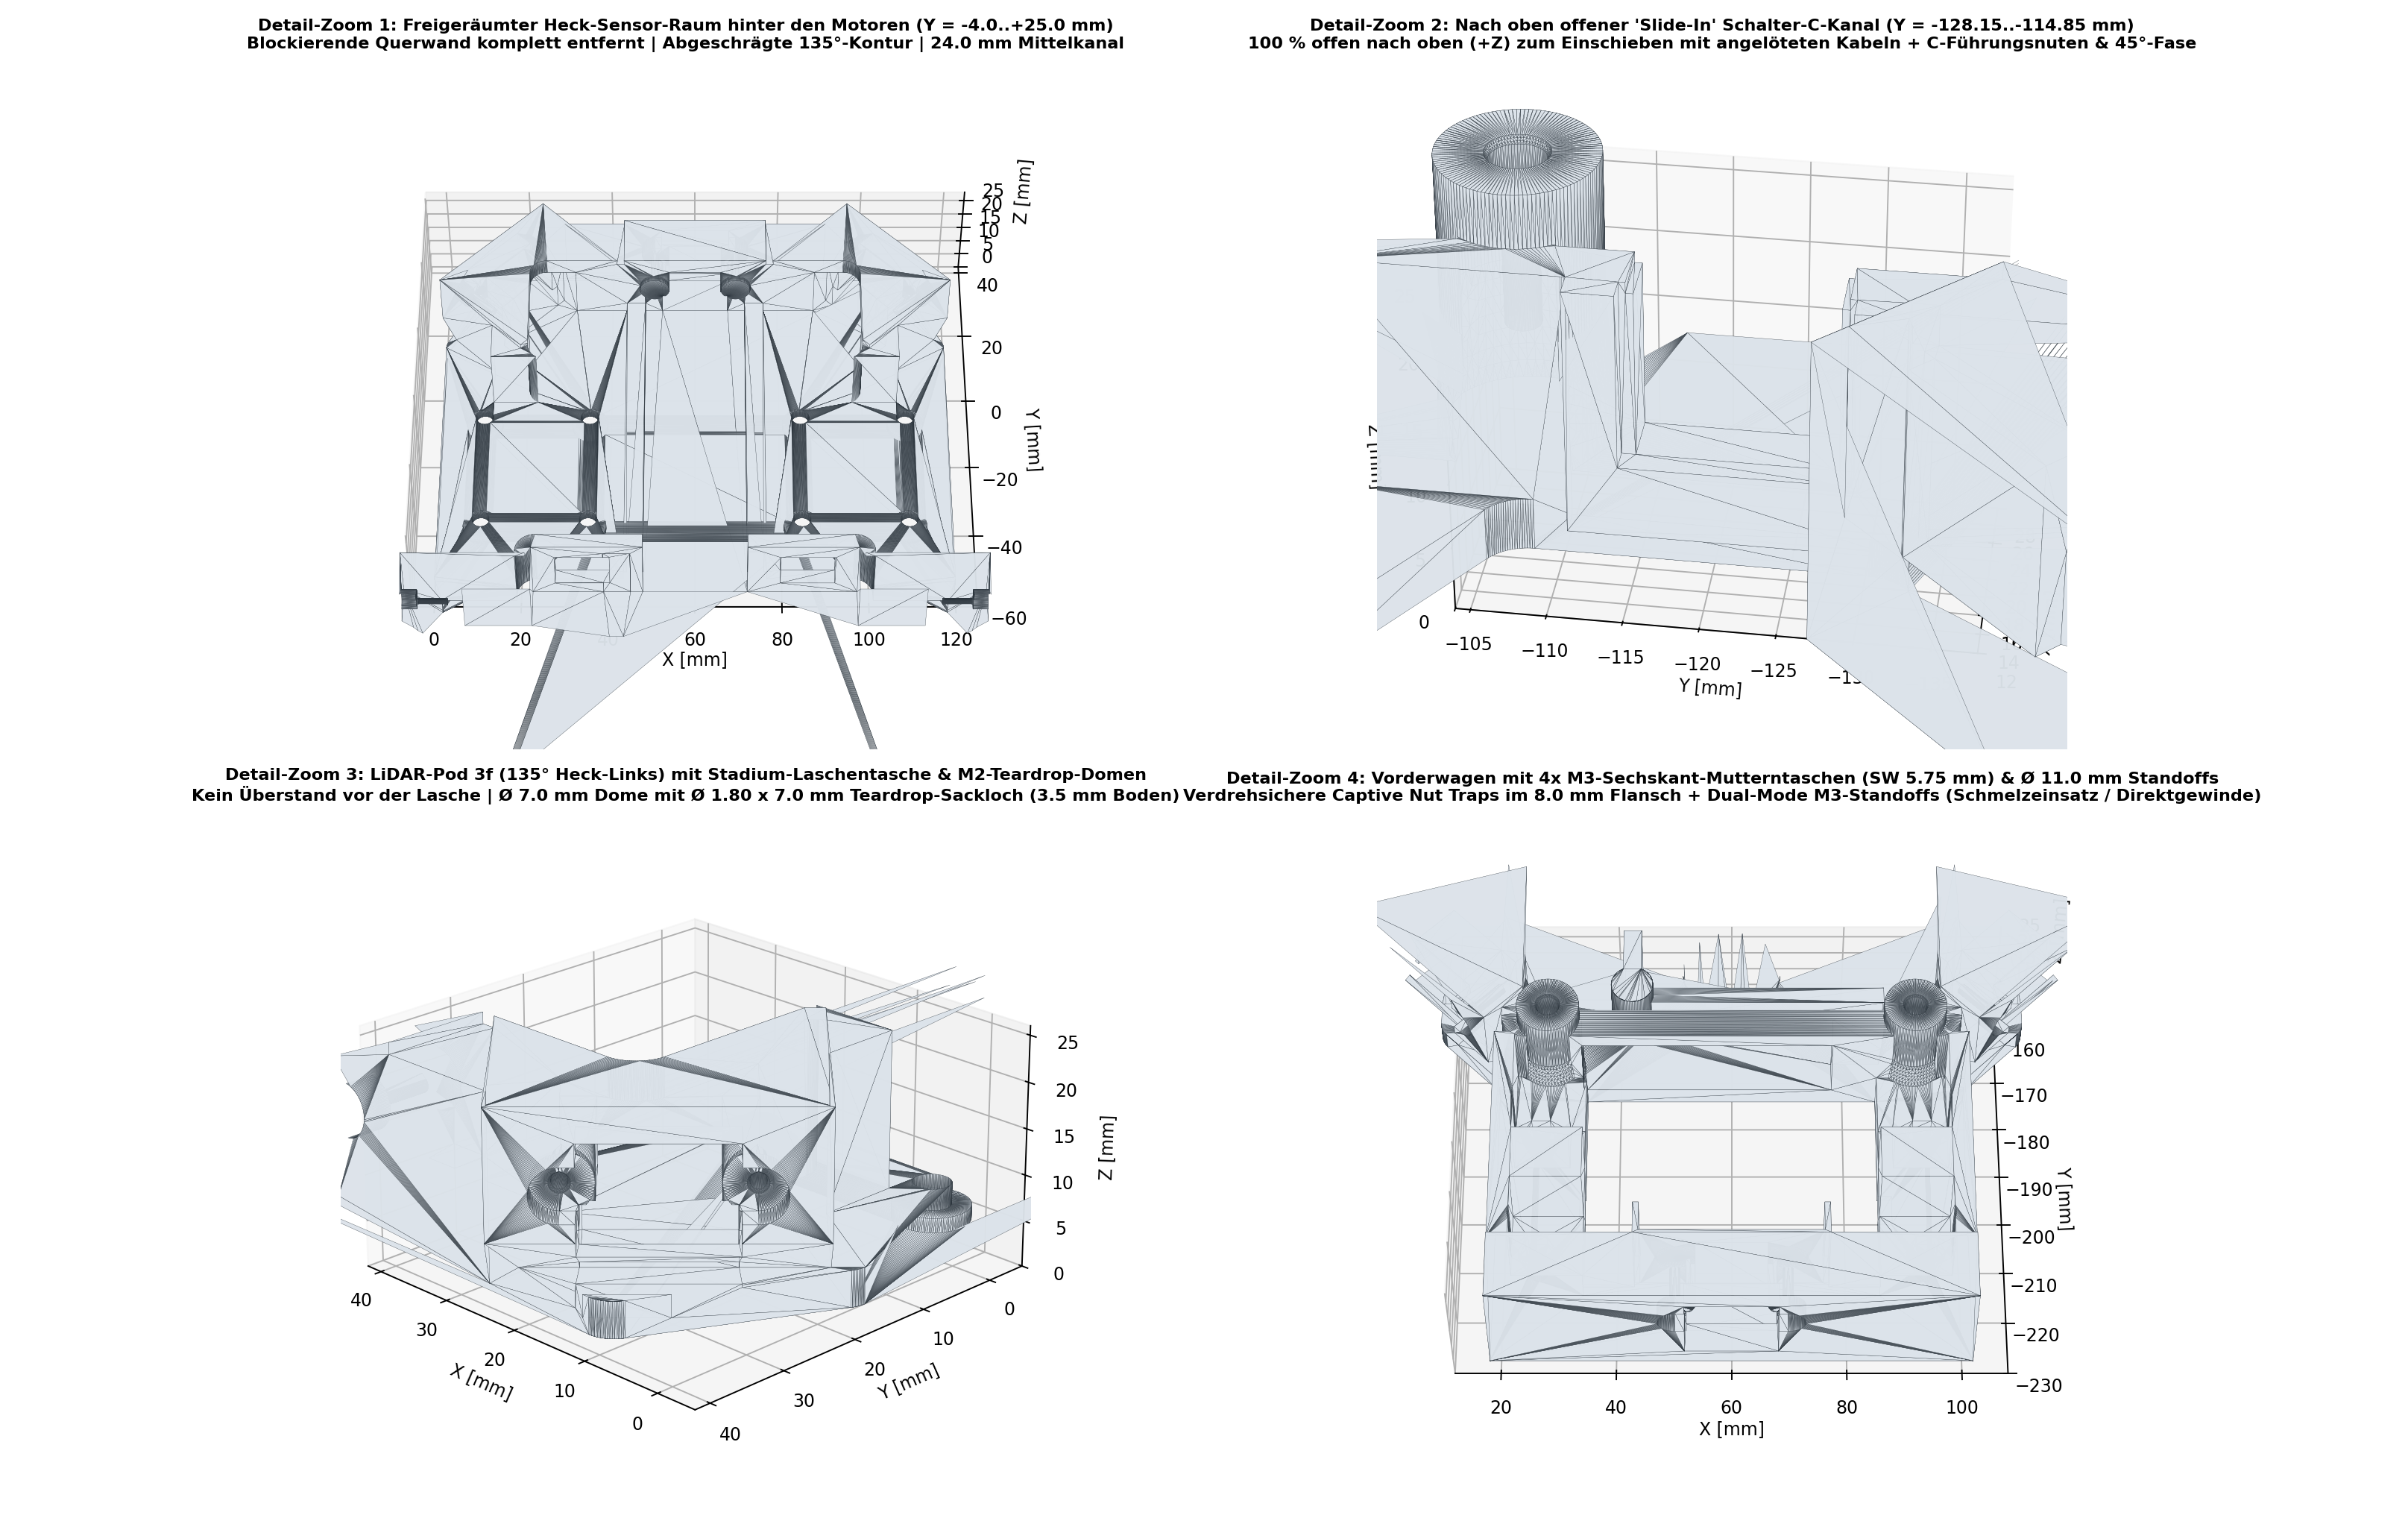
\includegraphics[width=0.98\textwidth]{figures/cad_v10_detail_zooms.png}
  \caption{Detail-Zooms des druckfertigen Chassis v10.0: (1) freigeräumter Heckbereich hinter den Motoren, (2) nach oben offener Slide-In-Schalterkanal, (3) 135°-Pod mit Stadium-Tasche und M2-Teardrop-Domen, (4) Vorderwagen mit vier M3-Sechskant-Mutterntaschen und Dual-Mode-Standoffs.}
  \label{fig:cad_v10_zooms}
\end{figure}

\begin{figure}[htbp]
  \centering
  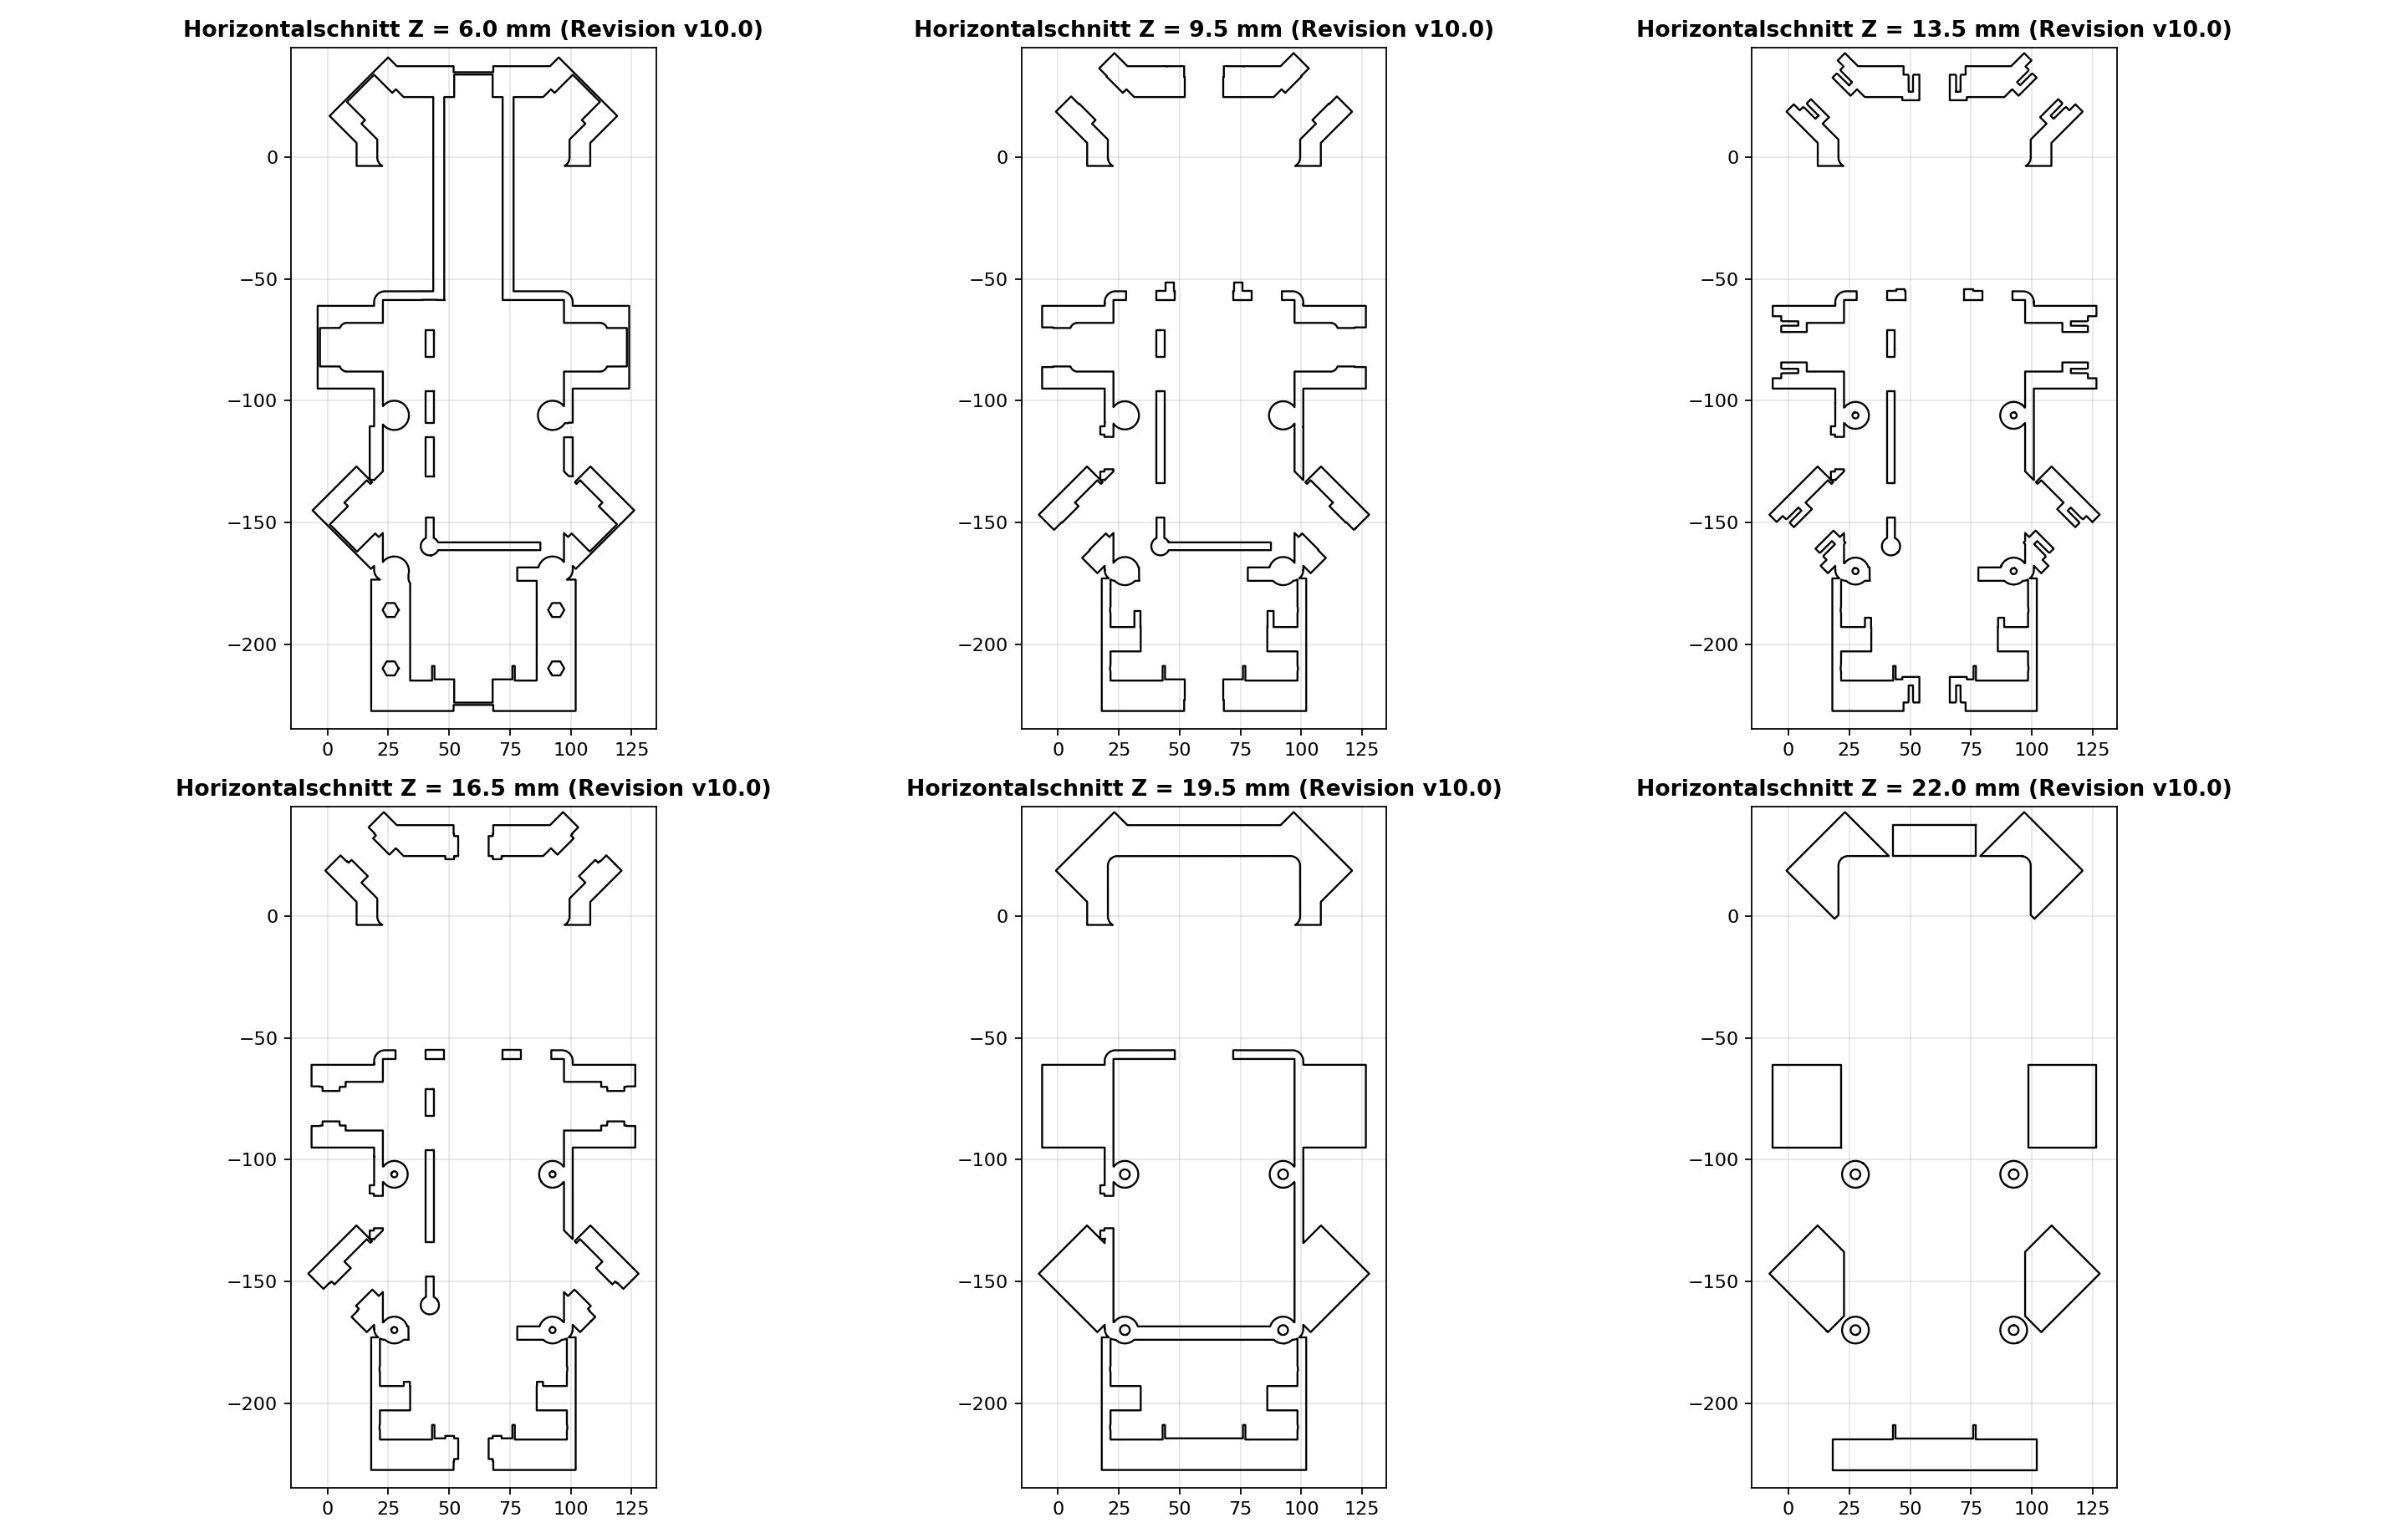
\includegraphics[width=0.98\textwidth]{figures/cad_v10_cross_sections.png}
  \caption{Horizontalschnitte des Chassis v10.0 von $Z = \qty{6,0}{\milli\meter}$ bis $Z = \qty{22,0}{\milli\meter}$: Nachweis der offenen Heck-Kabelwege, der durchgängigen 45°-/90°-Steckerkanäle, der Sechskant-Mutterntaschen ($Z = \qty{6,0}{\milli\meter}$) und der geschlossenen Pod-Decken ($Z = \qty{22,0}{\milli\meter}$).}
  \label{fig:cad_v10_slices}
\end{figure}

\subsection{Normgerechte Verbindungstechnik und DfAM für den Bambu Lab P1S}
Für eine dauerhafte, wiederholt lösbare Montage im 3D-gedruckten Kunststoff wurden alle 32 Schraubverbindungen gezielt nach \gls{dfam}-Regeln ausgelegt:
\begin{itemize}
  \item \textbf{4$\times$ Hauptplatinen-Standoffs (\texttt{H1}--\texttt{H4}, \diameter\,\qty{11,0}{\milli\meter}, Dual-Mode):} Oben befindet sich eine \diameter\,\qtyproduct{4,00 x 6,0}{\milli\meter} Bohrung mit \qty{0,6}{\milli\meter} Einführfase für M3-Messing-Einschmelzgewinde (\qty{3,50}{\milli\meter} radiale Restwandstärke). Direkt darunter liegt ein \diameter\,\qtyproduct{2,50 x 7,0}{\milli\meter} M3-Kernloch, sodass im Bedarfsfall auch ohne Schmelzeinsätze direkt mit M3$\times$12-Schrauben montiert werden kann (\qty{12,50}{\milli\meter} geschlossener Boden).
  \item \textbf{4$\times$ Liniensensor-Befestigung (Captive Hex Nut Traps):} In den \qty{8,0}{\milli\meter} starken Frontflanschen sind oberseitig vier verdrehsichere Sechskant-Mutterntaschen (Schlüsselweite \qty{5,75}{\milli\meter} für DIN-934-M3-Muttern mit \qty{0,25}{\milli\meter} FDM-Spiel, Tiefe \qty{2,80}{\milli\meter}, \qty{5,20}{\milli\meter} Flanschboden) integriert. Dadurch genügt ein einziger Innensechskantschlüssel von unten.
  \item \textbf{8$\times$ Motorhalter-Bohrungen:} \diameter\,\qty{4,20}{\milli\meter} Durchgangsbohrungen mit unterseitiger \diameter\,\qtyproduct{8,40 x 1,60}{\milli\meter} Senkung, damit die Köpfe der M4$\times$10-Senkschrauben bündig in der \qty{4,0}{\milli\meter} Bodenplatte verschwinden.
  \item \textbf{Akku-Fixierung:} Im rechten Batteriefach (\qtyproduct{78,0 x 43,3 x 21,5}{\milli\meter}, $+1{,}9$ bis $+\qty{3,0}{\milli\meter}$ Einbauspiel für das \qtyproduct{72,0 x 39,5 x 19,5}{\milli\meter} 2S-Pack) sind bei $Y = \qty{-112}{\milli\meter}$ und $Y = \qty{-134}{\milli\meter}$ durchgehende \qtyproduct{6,0 x 2,2}{\milli\meter} Klettband-Ösen integriert.
\end{itemize}

Für den Druck auf dem schuleigenen \emph{Bambu Lab P1S} (\qtyproduct{256 x 256 x 256}{\milli\meter} Bauraum \cite{BambuLab_P1S}) wurde ein wichtiger geometrischer Punkt berücksichtigt: Mit einer Gesamtlänge von \qty{270,36}{\milli\meter} überschreitet das Chassis bei \qty{0}{\degree}-Ausrichtung die Bettlänge um \qty{14,4}{\milli\meter}. Durch eine Rotation um $+\qty{45}{\degree}$ um die Z-Achse sinkt der umschreibende Quader jedoch auf exakt \qtyproduct{250,53 x 250,53 x 25,50}{\milli\meter} und lässt dabei sogar die vordere linke Filament-Cutter-Sperrzone des P1S komplett frei. Die Seitenwandstärke von \qty{3,60}{\milli\meter} entspricht exakt neun geschlossenen \qty{0,40}{\milli\meter}-Wandlinien, die \qty{4,00}{\milli\meter}-Bodenplatte exakt 20 Schichten bei \qty{0,20}{\milli\meter} Schichthöhe. Alle positiven Aufbauten wurden um \qty{1,0}{\milli\meter} in die Bodenplatte eingebettet, um koplanare OpenCASCADE-Kanten auszuschließen -- die automatische Prüfung mit \texttt{trimesh} bestätigt ein **100\,\% wasserdichtes (manifold) STL-Netz** (\texttt{is\_watertight = True}, 1 Festkörper, 54.556 Dreiecke, \qty{220,8}{\centi\meter\cubed}, ca. \qty{274}{\gram} Filament, \qty{0}{\gram} Stützmaterial).

\subsection{Mechanische Stoßfestigkeits-Abschätzung (Crash-Analyse)}
Um sicherzustellen, dass das Chassis bei einer ungewollten Wandkollision mit $v = \qty{5}{\kilo\meter\per\hour} \approx \qty{1,39}{\meter\per\second}$ (Gesamtmasse $m \approx \qty{1,20}{\kilo\gram}$) nicht bricht, wird die mittlere Stoßkraft $F_{\mathrm{Sto\ss}}$ über einen angenommenen elastisch-plastischen Bremsweg von $s = \qty{2,0}{\milli\meter}$ abgeschätzt:
\begin{equation}
  F_{\mathrm{Sto\ss}} = \frac{E_{\mathrm{kin}}}{s} = \frac{\frac{1}{2} \cdot m \cdot v^2}{s} = \frac{0{,}5 \cdot \qty{1,20}{\kilo\gram} \cdot (\qty{1,39}{\meter\per\second})^2}{\qty{0,002}{\meter}} \approx \qty{579}{\newton}
  \label{eq:crash_kraft}
\end{equation}
Die Kraft wird über den \qty{6,0}{\milli\meter} starken Front-Bumper direkt in die beiden \qtyproduct{16 x 8}{\milli\meter} Frontflansche, die beiden Längsstreben (\qtyproduct{10 x 13,5}{\milli\meter}) und die vorderen Versteifungs-Gussets eingeleitet ($A_{\mathrm{trag}} \approx \qty{618}{\milli\meter\squared}$). Damit ergibt sich eine mittlere Druckspannung von:
\begin{equation}
  \sigma_{\mathrm{Druck}} = \frac{F_{\mathrm{Sto\ss}}}{A_{\mathrm{trag}}} = \frac{\qty{579}{\newton}}{\qty{618}{\milli\meter\squared}} \approx \qty{0,94}{\mega\pascal}
  \label{eq:crash_spannung}
\end{equation}
Gegenüber der konservativen zulässigen Druckfestigkeit von FDM-PETG/PLA quer zur Schichtebene ($\sigma_{\mathrm{zul}} \approx \qty{35}{\mega\pascal}$) verbleibt ein sehr großer rechnerischer Sicherheitsfaktor ($\mathrm{SF} > 35$; selbst bei einer extremen Testgeschwindigkeit von \qty{9}{\kilo\meter\per\hour} liegt $\mathrm{SF} > 11$).

% ==============================================================================
\section{Gesamtstückliste (Hardware- und Normteile-BOM)}
\label{sec:bom}
% ==============================================================================
Tabelle~\ref{tab:bom_gesamt} fasst die wesentlichen elektronischen, elektromechanischen und mechanischen Komponenten inklusive der exakt abgestimmten Verbindungselemente zusammen. Die vollständige Einzelbauteil-BOM der Liniensensor-Platine (37 Positionen inkl. Hersteller-MPNs) befindet sich im Projektverzeichnis \texttt{PCB/Liniensensor\_Redesign/Stueckliste.csv}.

\begin{longtable}{@{}p{0.8cm}p{4.3cm}p{3.8cm}p{4.9cm}@{}}
\caption{Übersicht der Hauptkomponenten und Normteile des Tumbler~v3.0.}
\label{tab:bom_gesamt} \\
\toprule
\textbf{Anz.} & \textbf{Bauteil / Baugruppe} & \textbf{Typ / Spezifikation} & \textbf{Einsatzort / Bemerkung} \\
\midrule
\endfirsthead
\toprule
\textbf{Anz.} & \textbf{Bauteil / Baugruppe} & \textbf{Typ / Spezifikation} & \textbf{Einsatzort / Bemerkung} \\
\midrule
\endhead
\bottomrule
\endfoot
1 & Mikrocontroller-Modul & \emph{ESP32-S3-WROOM-1} & Hauptplatine (\texttt{U3}), Dual-Core \qty{240}{\mega\hertz} \\
2 & H-Brücken-Motortreiber & \emph{Toshiba TB67H450FNG} & Hauptplatine (\texttt{U6}, \texttt{U7}), bis \qty{3,5}{\ampere} \\
1 & 6-Achsen-IMU & \emph{ST LSM6DSV} (I\textsuperscript{2}C) & Hauptplatine (\texttt{U5}), Gierwinkel-Stützung \\
1 & Abwärtswandler & \emph{Diodes AP63203} & Effiziente \qty{5}{\volt}/\qty{3,3}{\volt}-Erzeugung \\
8 & Optische ToF-Sensoren & \emph{VL53L0/1XV2} (Breakout) & 360°-Sensorring (\texttt{3a}--\texttt{3h}), I\textsuperscript{2}C + XSHUT \\
6 & Optische Reflexkoppler & \emph{Vishay CNY70} & Liniensensor-Platine (\texttt{U1}--\texttt{U6}), \qty{10}{\milli\meter}-Raster \\
2 & NPN-Stromsenken & \emph{Nexperia BC817-40,215} & Liniensensor (\texttt{Q1}, \texttt{Q2}), SOT-23, $\approx \qty{20}{\milli\ampere}$ \\
1 & Steckverbinder-Set & \emph{JST GH} 10-pol. (\qty{1,25}{\milli\meter}) & \texttt{SM10B-GHS-TB} / \texttt{BM10B-GHS-TBT} (\texttt{J2}) \\
2 & DC-Getriebemotoren & \emph{GA37-520} + Encoder & Hinterachse mit 2$\times$ L-Winkel \& \diameter\,\qty{66}{\milli\meter} Rädern \\
1 & 2S-Li-Ion-Akkupack & \qty{7,4}{\volt} nom. (\qtyrange{6,4}{8,4}{\volt}) & \qtyproduct{72 x 39,5 x 19,5}{\milli\meter}, XT30 + Balancer \\
1 & Hauptschalter & Wippenschalter \qtyproduct{13 x 13}{\milli\meter} & Linker Slide-In-C-Kanal + Snap-On Clip \\
1 & Unibody-Chassis v10.0 & PETG/PLA (\qty{220,8}{\centi\meter\cubed}) & Bambu Lab P1S, \qty{0,2}{\milli\meter} Layer, 4 Wandlinien \\
16 & LiDAR-Schrauben & M2$\times$6 (oder M2$\times$8) ISO 4762 & Selbstfurchend in \diameter\,\qty{1,80}{\milli\meter} Teardrop-Dome \\
4 & PCB-Schrauben + Inserts & M3$\times$8 + M3$\times$5,7 Messing & Hauptplatine auf \texttt{H1}--\texttt{H4} (alt. M3$\times$12 direkt) \\
4 & Liniensensor-Schrauben & M3$\times$12 + M3-Mutter DIN 934 & Verdrehsicher in 4$\times$ Sechskant-Mutterntaschen \\
8 & Motorhalter-Schrauben & M4$\times$10 DIN 7991 + DIN 985 & Bündig versenkt in \qty{4,0}{\milli\meter} Bodenplatte \\
\end{longtable}
